%  LaTeX support: latex@mdpi.com 
%  For support, please attach all files needed for compiling as well as the log file, and specify your operating system, LaTeX version, and LaTeX editor.

%=================================================================
\documentclass[mathematics,article,submit,pdftex,moreauthors]{Definitions/mdpi} 
\usepackage[nolist,nohyperlinks]{acronym}
\usepackage{subcaption}
\usepackage{bm}
\nocite{*}
\renewcommand{\vec}[1]{\bm{#1}}

\begin{acronym}[SSCS]
    \acro{agp}[AGP]{automated gradual pruning}
    \acro{cnn}[CNN]{convolutional neural network}
    \acro{fcn}[FCN]{fully convolutional network}
    \acro{fpn}[FPN]{feature pyramid network}
    \acro{iou}[IoU]{intersection over union}
    \acro{lp}[LP]{linear pruning}
    \acro{manet}[MA-Net]{multi-scale attention network}
    \acro{mp}[MP]{movement pruning}
    \acro{nea}[NEA]{naturally eroded wall}
    \acro{relu}[ReLU]{rectified linear unit}
    \acro{resnet101}[ResNet-101]{101 layers residual network}
    \acro{sgd}[SGD]{stochastic gradient descent}
    \acro{sscs}[SSCS]{steel corrosion condition state}
    \acro{svm}[SVM]{support vector machine}
    \acro{uav}[UAV]{unmanned aerial vehicle}
\end{acronym}
%--------------------
% Class Options:
%--------------------
%----------
% journal
%----------
% Choose between the following MDPI journals:
% acoustics, actuators, addictions, admsci, adolescents, aerobiology, aerospace, agriculture, agriengineering, agrochemicals, agronomy, ai, air, algorithms, allergies, alloys, analytica, analytics, anatomia, animals, antibiotics, antibodies, antioxidants, applbiosci, appliedchem, appliedmath, applmech, applmicrobiol, applnano, applsci, aquacj, architecture, arm, arthropoda, arts, asc, asi, astronomy, atmosphere, atoms, audiolres, automation, axioms, bacteria, batteries, bdcc, behavsci, beverages, biochem, bioengineering, biologics, biology, biomass, biomechanics, biomed, biomedicines, biomedinformatics, biomimetics, biomolecules, biophysica, biosensors, biotech, birds, bloods, blsf, brainsci, breath, buildings, businesses, cancers, carbon, cardiogenetics, catalysts, cells, ceramics, challenges, chemengineering, chemistry, chemosensors, chemproc, children, chips, cimb, civileng, cleantechnol, climate, clinpract, clockssleep, cmd, coasts, coatings, colloids, colorants, commodities, compounds, computation, computers, condensedmatter, conservation, constrmater, cosmetics, covid, crops, cryptography, crystals, csmf, ctn, curroncol, cyber, dairy, data, ddc, dentistry, dermato, dermatopathology, designs, devices, diabetology, diagnostics, dietetics, digital, disabilities, diseases, diversity, dna, drones, dynamics, earth, ebj, ecologies, econometrics, economies, education, ejihpe, electricity, electrochem, electronicmat, electronics, encyclopedia, endocrines, energies, eng, engproc, entomology, entropy, environments, environsciproc, epidemiologia, epigenomes, est, fermentation, fibers, fintech, fire, fishes, fluids, foods, forecasting, forensicsci, forests, foundations, fractalfract, fuels, future, futureinternet, futurepharmacol, futurephys, futuretransp, galaxies, games, gases, gastroent, gastrointestdisord, gels, genealogy, genes, geographies, geohazards, geomatics, geosciences, geotechnics, geriatrics, grasses, gucdd, hazardousmatters, healthcare, hearts, hemato, hematolrep, heritage, higheredu, highthroughput, histories, horticulturae, hospitals, humanities, humans, hydrobiology, hydrogen, hydrology, hygiene, idr, ijerph, ijfs, ijgi, ijms, ijns, ijpb, ijtm, ijtpp, ime, immuno, informatics, information, infrastructures, inorganics, insects, instruments, inventions, iot, j, jal, jcdd, jcm, jcp, jcs, jcto, jdb, jeta, jfb, jfmk, jimaging, jintelligence, jlpea, jmmp, jmp, jmse, jne, jnt, jof, joitmc, jor, journalmedia, jox, jpm, jrfm, jsan, jtaer, jvd, jzbg, kidneydial, kinasesphosphatases, knowledge, land, languages, laws, life, liquids, literature, livers, logics, logistics, lubricants, lymphatics, machines, macromol, magnetism, magnetochemistry, make, marinedrugs, materials, materproc, mathematics, mca, measurements, medicina, medicines, medsci, membranes, merits, metabolites, metals, meteorology, methane, metrology, micro, microarrays, microbiolres, micromachines, microorganisms, microplastics, minerals, mining, modelling, molbank, molecules, mps, msf, mti, muscles, nanoenergyadv, nanomanufacturing,\gdef\@continuouspages{yes}} nanomaterials, ncrna, ndt, network, neuroglia, neurolint, neurosci, nitrogen, notspecified, %%nri, nursrep, nutraceuticals, nutrients, obesities, oceans, ohbm, onco, %oncopathology, optics, oral, organics, organoids, osteology, oxygen, parasites, parasitologia, particles, pathogens, pathophysiology, pediatrrep, pharmaceuticals, pharmaceutics, pharmacoepidemiology,\gdef\@ISSN{2813-0618}\gdef\@continuous pharmacy, philosophies, photochem, photonics, phycology, physchem, physics, physiologia, plants, plasma, platforms, pollutants, polymers, polysaccharides, poultry, powders, preprints, proceedings, processes, prosthesis, proteomes, psf, psych, psychiatryint, psychoactives, publications, quantumrep, quaternary, qubs, radiation, reactions, receptors, recycling, regeneration, religions, remotesensing, reports, reprodmed, resources, rheumato, risks, robotics, ruminants, safety, sci, scipharm, sclerosis, seeds, sensors, separations, sexes, signals, sinusitis, skins, smartcities, sna, societies, socsci, software, soilsystems, solar, solids, spectroscj, sports, standards, stats, std, stresses, surfaces, surgeries, suschem, sustainability, symmetry, synbio, systems, targets, taxonomy, technologies, telecom, test, textiles, thalassrep, thermo, tomography, tourismhosp, toxics, toxins, transplantology, transportation, traumacare, traumas, tropicalmed, universe, urbansci, uro, vaccines, vehicles, venereology, vetsci, vibration, virtualworlds, viruses, vision, waste, water, wem, wevj, wind, women, world, youth, zoonoticdis 
% For posting an early version of this manuscript as a preprint, you may use "preprints" as the journal. Changing "submit" to "accept" before posting will remove line numbers.

%---------
% article
%---------
% The default type of manuscript is "article", but can be replaced by: 
% abstract, addendum, article, book, bookreview, briefreport, casereport, comment, commentary, communication, conferenceproceedings, correction, conferencereport, entry, expressionofconcern, extendedabstract, datadescriptor, editorial, essay, erratum, hypothesis, interestingimage, obituary, opinion, projectreport, reply, retraction, review, perspective, protocol, shortnote, studyprotocol, systematicreview, supfile, technicalnote, viewpoint, guidelines, registeredreport, tutorial
% supfile = supplementary materials

%----------
% submit
%----------
% The class option "submit" will be changed to "accept" by the Editorial Office when the paper is accepted. This will only make changes to the frontpage (e.g., the logo of the journal will get visible), the headings, and the copyright information. Also, line numbering will be removed. Journal info and pagination for accepted papers will also be assigned by the Editorial Office.

%------------------
% moreauthors
%------------------
% If there is only one author the class option oneauthor should be used. Otherwise use the class option moreauthors.

%---------
% pdftex
%---------
% The option pdftex is for use with pdfLaTeX. Remove "pdftex" for (1) compiling with LaTeX & dvi2pdf (if eps figures are used) or for (2) compiling with XeLaTeX.

%=================================================================
% MDPI internal commands - do not modify
\firstpage{1} 
\makeatletter 
\setcounter{page}{\@firstpage} 
\makeatother
\pubvolume{1}
\issuenum{1}
\articlenumber{0}
\pubyear{2024}
\copyrightyear{2024}
%\externaleditor{Academic Editor: Firstname Lastname}
\datereceived{ } 
\daterevised{ } % Comment out if no revised date
\dateaccepted{ } 
\datepublished{ } 
%\datecorrected{} % For corrected papers: "Corrected: XXX" date in the original paper.
%\dateretracted{} % For corrected papers: "Retracted: XXX" date in the original paper.
\hreflink{https://doi.org/} % If needed use \linebreak
%\doinum{}
%\pdfoutput=1 % Uncommented for upload to arXiv.org
%\CorrStatement{yes}  % For updates


%=================================================================
% Add packages and commands here. The following packages are loaded in our class file: fontenc, inputenc, calc, indentfirst, fancyhdr, graphicx, epstopdf, lastpage, ifthen, float, amsmath, amssymb, lineno, setspace, enumitem, mathpazo, booktabs, titlesec, etoolbox, tabto, xcolor, colortbl, soul, multirow, microtype, tikz, totcount, changepage, attrib, upgreek, array, tabularx, pbox, ragged2e, tocloft, marginnote, marginfix, enotez, amsthm, natbib, hyperref, cleveref, scrextend, url, geometry, newfloat, caption, draftwatermark, seqsplit
% cleveref: load \crefname definitions after \begin{document}

%=================================================================
% Please use the following mathematics environments: Theorem, Lemma, Corollary, Proposition, Characterization, Property, Problem, Example, ExamplesandDefinitions, Hypothesis, Remark, Definition, Notation, Assumption
%% For proofs, please use the proof environment (the amsthm package is loaded by the MDPI class).

%=================================================================
% Full title of the paper (Capitalized)
\Title{Neural Network Pruning for Lightweight Metal Corrosion 
Image Segmentation Models}

% MDPI internal command: Title for citation in the left column
\TitleCitation{Title}

% Author Orchid ID: enter ID or remove command
\newcommand{\orcidauthorA}{0000-0000-0000-000X} % Add \orcidA{} behind the author's name
%\newcommand{\orcidauthorB}{0000-0000-0000-000X} % Add \orcidB{} behind the author's name

% Authors, for the paper (add full first names)
\Author{Firstname Lastname $^{1,\dagger,\ddagger}$\orcidA{}, Firstname Lastname $^{2,\ddagger}$ and Firstname Lastname $^{2,}$*}

%\longauthorlist{yes}

% MDPI internal command: Authors, for metadata in PDF
\AuthorNames{Firstname Lastname, Firstname Lastname and Firstname Lastname}

% MDPI internal command: Authors, for citation in the left column
\AuthorCitation{Lastname, F.; Lastname, F.; Lastname, F.}
% If this is a Chicago style journal: Lastname, Firstname, Firstname Lastname, and Firstname Lastname.

% Affiliations / Addresses (Add [1] after \address if there is only one affiliation.)
\address{%
$^{1}$ \quad Affiliation 1; e-mail@e-mail.com\\
$^{2}$ \quad Affiliation 2; e-mail@e-mail.com}

% Contact information of the corresponding author
\corres{Correspondence: e-mail@e-mail.com; Tel.: (optional; include country code; if there are multiple corresponding authors, add author initials) +xx-xxxx-xxx-xxxx (F.L.)}

% Current address and/or shared authorship
\firstnote{Current address: Affiliation.}  % Current address should not be the same as any items in the Affiliation section.
\secondnote{These authors contributed equally to this work.}
% The commands \thirdnote{} till \eighthnote{} are available for further notes

%\simplesumm{} % Simple summary

%\conference{} % An extended version of a conference paper

\abstract{The threat of metal corrosion is
a critical concern across various industries,
as it can lead to structural failures, safety risks, and significant economic losses.
Therefore, effective
inspection is paramount in early detection 
metal corrosion.
Recently, computer vision methods,
especially deep learning (DL)-based methods,
for aiding visual detection of metal corrosion have
been gaining popularity. DL-based methods
not only make the inspection more efficient,
but also maintain high accuracy in corrosion detection.
Although DL-based methods offer promising enhancement
to the inspection tasks, one needs to consider
its high computational requirements, especially
for deploying them in remote areas where only
resource-constrained devices, e.g., edge devices
are affordable. Therefore, it is essential
to develop lightweight DL models that can be 
deployed on edge devices, ensuring efficient
corrosion detection even in resource-constrained environments.
This study proposes to develop lightweight DL models
for metal corrosion segmentation by pruning the models.
The aim of pruning is to remove
redundant parameters, thus reducing the size
and computational load, without
compromising much on performance. In this study,
we evaluate five image segmentation models, i.e., 
U-Net, U-Net++, FPN, LinkNet and MA-Net,
and three pruning algorithms, i.e., 
linear, AGP and movement pruning, on two metal corrosion
image segmentation datasets, i.e., NEA and SSCS datasets. 
The conducted experimental study shows that we can train
the models, e.g., FPN, and prune the model
up to  $90\%$ sparsity with less than $10\%$
IoU reduction on SSCS dataset and less than
$5\%$ IoU reduction on NEA dataset.}

\keyword{keyword 1; keyword 2; keyword 3 (List three to ten pertinent keywords specific to the article; yet reasonably common within the subject discipline.)} 

% The fields PACS, MSC, and JEL may be left empty or commented out if not applicable
%\PACS{J0101}
%\MSC{}
%\JEL{}

%%%%%%%%%%%%%%%%%%%%%%%%%%%%%%%%%%%%%%%%%%
\begin{document}

%%%%%%%%%%%%%%%%%%%%%%%%%%%%%%%%%%%%%%%%%%
\section{Introduction}

Metal corrosion is an ever-present problem in maintaiing 
infrastructures globally. If left undetected
and unattended, corrosion can cause serious damage to the infrastructures
resulting in premature end-of-life of the infrastructures,
direct and indirect financial loss, 
and ultimately poses critical safety risks. It 
is no wonder that the global cost estimates of
corrosion is \$25 trillion~\cite{Koch2016}.
Therefore, it is imperative to
inspect infrastructures for metallic corrosion
regularly. Corrosion detection and maintance
are vtial to prevent metallic corrosion~\cite{Wang2019}.

Commonly, corrosion detection is conducted 
visually by experts on the field. The inspection is 
also conducted on images collected by \ac{uav}, especially
on hard-to-reach parts of the structure.
Afterward, the collected images are analyzed to detect
the corrosion. Nowadays, various computer-based
methods have been proposed to detect corrosion
from these images. The methods range from
tradional image processing techniques,
e.g., color space based detection~\cite{Igoe2016} 
and texture analysis-based detection~\cite{Pascual2014},
to machine learning-based methods, e.g.,
\ac{svm}~\cite{Chen2012} and various 
\ac{cnn}-based models~\cite{Nash2022, Liu2023}.
Deep learning-based methods have been gaining more
popular due to its faster process while achieving
even pixel-level accuracy. 

Despite its qualities, one also need to consider
the required computational resources, including
financial cost, networking and accessability,
in deploying deep-learning based solutions.
This is even more important when one wants to 
deploy deep learning-based solutions in remote
areas where only edge devices can be afforded.
Therefore, to reduce computational resource requirements
of these methods, lightweight 
models can be a solution for these limitations.

In this study, we propose to produce lightweight
models for multiclass image segmentation
task for pixel level metal corrosion detection.
We make the models lightweight by pruning the neural 
network's weights. We propose to prepare the lightweight models
by training the models, pruning their weights, followed
by fine-tuning the pruned models. 
In this study,
we experimentally evaluate five neural network
architectures, i.e., \ac{fpn}~\cite{Lin2017}, U-NET~\cite{Ronneberger2015},
U-NET++~\cite{Zhou2018}, \ac{manet}~\cite{Fan2020}, and 
LinkNet~\cite{Chaurasia2017}. For each of these architectures,
we employ \ac{resnet101}~\cite{He2016} pretrained on ImageNet
dataset as the feature extractor. Thre pruning strategies
are considered in the pruning stage, namely
\ac{lp}, \ac{agp} algorithm~\cite{Han2017},
and \ac{mp} algorithm~\cite{Sanh2020}. We prune
the models up to $90\%$ sparsity and 
evaluate their performance based on their
achieved \ac{iou}. The methods
are evaluated on two metal corrosion image datasets,
i.e., the \ac{sscs} dataset \cite{Bianchi2021Dataset,Bianchi2022Journal} and 
the \ac{nea} dataset \cite{Liu2023}. 


\section{Methods}
This section describes the considered architectures,
the pruning algorithms, and the datasets. Before that,
we briefly describe the loss function used to 
train the models and the \ac{iou} metric.
Throughout all stages, the models are trained to minimize
the Tversky loss function~\cite{Salehi2017} as given
by:
\begin{equation}
    L(\hat{\alpha}, \hat{\beta}) = \frac{\text{TP}}{\text{TP}+
    \hat{\alpha}\text{FP} +  \hat{\beta}\text{FN}},
\end{equation}
where TP denotes the true positives, FP the false positives
and FN the false negatives. The two hyperparameters of 
the loss function are $\hat{\alpha}$ and $\hat{\beta}$
that adjust the trade-off between false positives and
false negatives. The metric used to evalute the performance of the trained
models is the \ac{iou}, which is given by:
\begin{equation}
    IoU = \frac{\text{TP}}{\text{TP}+\text{FP}+\text{FN}}.
\end{equation}


\subsection{Architectures}

U-NET~\cite{Ronneberger2015} is an extension to
 \ac{fcn}~\cite{Long2015} where the architecture
 comprises two parts, the left contracting path
 and the right expanding path. The contracting
 path is a repeated component comprising two $3\times 3$
 unpadded convolutions, a \ac{relu}, and a $2\times 2 $ max
 pooling layer with stride 2 for downsampling. The
 number of feature channes is double at each downsampling
 step. Similarly, the expanding path is also 
 repeated components comprising feature map unsampling,
 $2\times 2$ convolutions to halve the number of feature channels, 
 a concatenation with the cropped feature map from
 the contracting part, and two $3\times 3$ convolutions
 each followed by a \ac{relu}. In total, the network
 has 23 convolutional layers.

U-Net++~\cite{Zhou2018} extends U-Net by adding a dense
network of skip connections between the contracting
and expanding paths. This extension is based on 
DenseNet~\cite{Huang2017}. Instead of directly concatenating
the feature maps from the contracting path onto the corresponding
layers in the exapnsive path, as is done in U-Net, U-Net++
has several skip connections between the corresponding layers.
Each skip connection unit takes the features map from the all
previous units at the same level and the upsampled feature map
for its immediate lower unit. The addition of these
skip connections minimize the loss of semantic information
between the two paths.

\ac{manet}~\cite{Fan2020} also extends U-Net by integrating
skip-connections and, more importantly, the self-attention mechanism.
Two new blocks based on self-attention mechanism, i.e., 
position-wise attention block in the bottleneck
part (in-between the contracting and expanding paths),
and multi-scale fusion attention block in the expanding
path, are proposed to capture spatial and channel
dependencies of the feature maps. The proposed dual
attention mechanism enhances the feature representation ability
of the model resulting in better performance
of the model for liver and tumor segmentation
task compared to other state-of-the-art models,
e.g., U-Net, U-Net++, and Densely \ac{fcn}~\cite{Krishna2018}.

Similary to the previous U-Net-based architectures,
\ac{fpn}~\cite{Lin2017} can also basically 
be divided into two pahts, the bottom-up path,
and the top-down path. The bottom-up
path computes a feature hierarchi consisting
of several scaled feature maps with a scaling
step of two. The path comprises several network
\textit{stages}, each stage consists of multiple layers
producing output maps of the same size.
Each stage equals one pyramid level in \ac{fpn}.
The top-down path generates higher resolution
features by upsampling the feature maps from
the higher pyramid levels, resulting
in spatially coarser but semantically stronger feature maps
compared to the higher pyramid levels.
The resulted features are combined with
the feature from the bottom-up
path of the same pyramid level through a lateral
connection. The design of \ac{fpn}
is flexible in the choice of module
for the building blocks.
However, the experimental evaluation in 
\cite{Lin2017} on varying the modules only
shows marginal difference in the resulted model's
performance. Therefore, similar to the original study,
this study opts for the simple design choice.

LinkNet~\cite{Chaurasia2017} also comprises two parts similar
to an encoder-decoder structure. 
The encoder and decoder are further
divided into several levels.
The encoder employed in LinkNet is a pre-trained
network, e.g., ResNet18 that
efficiently extracts high-level features from
the input. The decoder upsamples the feature
to its original size using transposed
convolutions. The output of the
encoder is combined with the input
to the decoder of the same level via
a residual network. The use of lightweight
pretrained encoder block and smaller
number of parameters compared to, e.g., 
U-Net-based architectures, results 
in a more efficient model without
majorly sacrificing its performance,
making LinkNet suitable for real-time
tasks.


\subsection{Pruning algorithms}
In this study, we evaluate three pruning algorithms, i.e., 
\ac{lp} algorithm, \ac{agp} algorithm~\cite{Han2017},
and \ac{mp} algorithm~\cite{Sanh2020}. Before
describing the three algorithms, we briefly discuss
the common notation of pruning neural network. 
Let $\vec{W}, |\vec{W}|=d$ be
the weight or parameters of a given model,
and $d$ is the number of the parameters. A
binary mask $\vec{M}, |\vec{M}|=d,$
is applied to $\vec{W}$ so that the output of
the model becomes:
\begin{equation}
    \vec{y} = (\vec{W} \odot \vec{M})\vec{x}, 
\end{equation}
where $\odot$ is the Hadamard or element-wise product.
The zero-ed out elements in $\vec{W}$ as a result
of the mask application is denoted
as the pruned weights. The binary mask 
is commonly computed based on a score $\vec{S}$
with its element correspond to each element of $\vec{M}$.
One of the method to compute $\vec{M}$ based on $\vec{S}$
is:
\begin{equation}
    M_i = \begin{cases}
        1, &\text{if } S_i \text{ in the top } \zeta\% \\
        0, &\text{otherwise,}
    \end{cases}
\end{equation}
with  $\zeta$ is the desired sparsity ratio of the model's
parameters.


These pruning algorithms
are gradual pruning algorithms, i.e., 
they increase the sparsity of the model weights gradually.
\ac{lp} is the most basic pruning algorithm where the
sparsity of the neural network at hand will be increased
linearly throughout the pruning phase.
The target sparsity increases linearly as given by:
\begin{equation}
    \zeta(t) = \zeta_0 + \frac{t-t_0}{n_p \Delta t} \zeta_f,
\end{equation}
with $\zeta(t)$ the target sparsity at the $t$-th 
training iteration, $n_p$ the total number of pruning steps, 
$\Delta t$ the training iteration interval between
two pruning steps, $t_0$ the starting training iteration,
 $\zeta_f$ the final target sparsity, and $\zeta_i$ the initial
sparsity which is usually $\zeta_0=0$.
One training iteration means one update step of the model's weights,
which commonly comprises one forward and backward pass, and 
one update step of the optimizer. 

\ac{agp} is similar to \ac{lp}, but it uses cubic sparsity
schedule to calculate the target sparsity, as given by:
\begin{equation}
    \zeta(t) = \zeta_f + (\zeta_0-\zeta_f)(1-\frac{t-t_0}{\Delta t n_p})^3.
\label{eq:methods:pruning:agp}
\end{equation}
Calculating the target sparsity using \eqref{eq:methods:pruning:agp}
results in more pruned weights at the early training iterations
when there are expected to be more redundant connections
compared to the later pruning stage. 

Various immediate pruning methods (as opposed to gradual)
can be employed at every pruning steps of \ac{lp}
and \ac{agp}. In this study, we use the Taylor
pruning method \cite{Molchanov2019}. This method
compute the importance of a parameter, say $W_i$,
based on the difference between the prediction errors
produced by the model with and without that parameter,
as given by:
\begin{equation}
    \mathcal{I}_{i}(W) = \left( E(\mathcal{D}, \vec{W}) - E(\mathcal{D}, W \mid W_i=0) \right)^2.
\end{equation}
To avoid the expensive computation of evaluating 
$|\vec{W}|$ different versions of the model, then
the difference can be approximated using the first-order
Taylor expansion as:
\begin{equation}
    \mathcal{I}^{(1)}_{i}(W) \triangleq \left( g_i W_i \right)^2,
\end{equation}
with $g_i = \frac{\delta E}{\delta W_i}$ is the $i$-th
element of the gradient $\vec{g}$. To approximate
the joint importance of a set of parameters,
say $\mathcal{I}^{(1)}_P(\vec{W}) \triangleq \sum_{j \in P} 
\mathcal{I}^{(1)}_{j}(W)$, with $P = \{j_1,\ldots, j_{|P|}\},
\forall j \in P, 0\leq j\leq |W|$.

Lastly, we briefly describe \ac{mp}. 
While most pruning algorithms retain the parameters
that are far from zero, \ac{mp} retains the parameters
that are moving away from zero. Based on this,
it can be denoted that \ac{mp} derived
the importance of parameters from the first-order
information instead of the zeroth-order information.
The score variable $\vec{S}$ now accumulates this movement
of the parameters after $t'$ training iterations as given by:
\begin{equation}
    S^{(t')}_i = - \alpha_S \sum_{t<t'} \left(\frac{\delta L}{\delta W_i}\right)^{(t)} W^{(t)}_i,
\end{equation}
where $L$ is the employed loss function, and $\vec{W}^{(t)}$ is the
model parameters at the $t$-th training iteration. The schedule
of sparsity level for each training iteration in \ac{mp}
is the same as \ac{agp}, i.e., as given by \eqref{eq:methods:pruning:agp}.


\subsection{Datasets}
In this study, the models are trained and evaluated on two metal corrosion image
datasets, namely, the \ac{sscs} dataset \cite{Bianchi2021Dataset,Bianchi2022Journal} and 
the \ac{nea} dataset \cite{Liu2023}. \ac{sscs} is a set of 
images from the structural inspection domain,
especially from the bridge inspection report 
by the Virginia Department of Transportation. 
The dataset comprises 440 annotated steel corrosion condition state images,
which are split into 396 training images and 44 testing images.
The corrosion state in the images are split into four corrosion
class categories, i.e., good (background), fair, poor and severe corrosion state.
An example of the image and its corresponding labels
from \ac{sscs} dataset is depicted in Figure~\ref{fig:dataset:ccsc-example}.
These images are resized into $512\times 512$ images in this study, as is also done
in the original paper \cite{Bianchi2022Journal}.

\begin{figure}[htbp]
    \begin{center}
    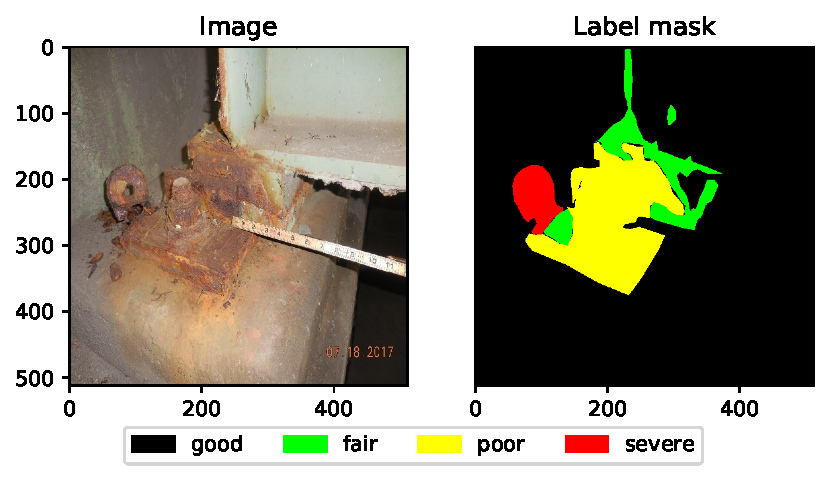
\includegraphics[width=0.5\textwidth]{figures/ccsc-example.pdf}
    \caption{An example of \ac{sscs} image and its corresponding label mask}
    \label{fig:dataset:ccsc-example}
    \end{center}
\end{figure}

\ac{nea} dataset comprises images of corroded metal wall
in natural environment collected by a \ac{uav}.
The dataset comprises 292 images of size $1280\times 720$.
The annotations comprise three class categories; one no corrosion class
and two corrosion classes. Unfortunately ,the difference
between the two corrosion classes is not clearly stated. 
In the original study \cite{Liu2023}, the authors
do not differentiate between the two corrosion class,
thus rendering the task as a binary semantic segmentation
task. However, in this study, 
we assume that one class is for poor corrosion state, 
while the other is for severe corrosion state, as shown
in Figure~\ref{fig:dataset:nea-example}. Therefore,
this study uses \ac{nea} dataset for a multiclass semantic
segmentation task.

\begin{figure}[htbp]
    \begin{center}
    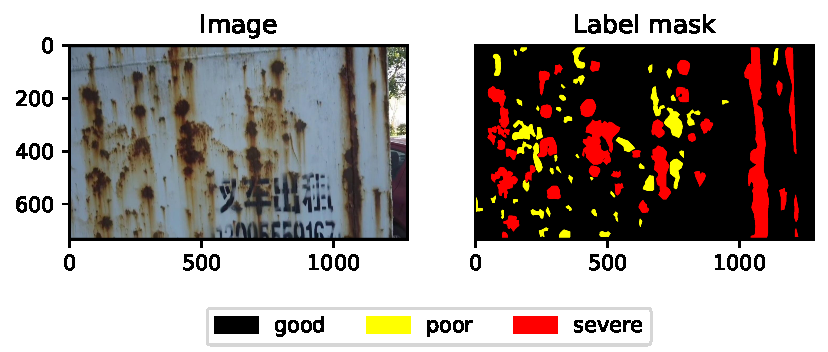
\includegraphics[width=0.5\textwidth]{figures/nea-example.pdf}
    \caption{An example of \ac{nea} image and its corresponding label mask}
    \label{fig:dataset:nea-example}
    \end{center}
\end{figure}


\subsection{Experimental settings}
All of the experiments are conducted on a 
single NVIDIA GeForce GTX 2080 Ti and
Intel i9-7900X with 20 cores. The source code in Pytorch is 
available at (github link provided before publishing).

In this experimental study, we use \ac{sgd} with
momentum as the optimizer and cyclical learning
rate scheduler~\cite{Smith2017}.
The momentum of the \ac{sgd} optimizer is set to 0.5
and the batch size is set to 4.
In addition, the hyperparameters for the cyclical learning
rate scheduler is set to $lr^{\min}_0=0.0001, lr^{\max}_0=0.01$ 
and $\delta_t=2000$. The hyperparameters for the optimizer and 
the learning rate scheduler are the same for the first
training stage, the pruning stage and the fine-tuning stage.

In the first training stage, the models
will be trained for $T=100$ epochs. In the pruning stage,
the models will be pruned for $T_{\text{pruning}}=50$ epochs.
Afterward, the pruned models will be fine-tuned for another 
$T_{\text{tuning}}=100$ epochs. For \ac{mp} algorithm,
we set $t_i=\frac{20N}{4}$ iterations and $t_f=\frac{10N}{4}$.
For the linear and \ac{agp} algorithms, the pruning
is done gradually in interval of ten epochs, thus the pruning
will be done five times in the span of $T_{\text{pruning}}=50$ epochs.

Throughout all training stages,
the training set will be split into two, $80\%$ for the 
training and $20\%$ for validation. The data augmentation
methods applied to the training dataset are affine operations,
flipping, rotation, scaling, and random cropping.
The target final sparsity we evaluate in this study
is $\zeta_f \in \{0.2, 0.5, 0.9\}$. We will evaluate the performance
of each combination of model, pruning algorithm, and
target sparsity based on the achieved \ac{iou} on
the testing dataset. In total there are $5\times 3\times 3=45$
combinations evaluated in this experimental study.

\section {Results and Discussion}
We describe the progress of the first
training stage. The validation \ac{iou}
obtained by the models throughout the epochs
of training is shown in 
Figure~\ref{fig:results:training:iou}.
The faded curve is the actual value, while the 
the bold curve is the exponential moving average
values with $\alpha=0.1$. The figure shows that
starting from around the 50-th epoch, the \ac{iou}
obtained by the models has plateaud.
The learning progress of \ac{fpn} is more stable
compared to other models, as it shows smaller variance
and it started with higher \ac{iou} compared to the other models.
On the other hand, other models showed great improvement
throughout the training progress as their starting \ac{iou}
is very small, even less than $0.1$ for LinkNet and U-Net
on \ac{sscs} dataset.

\begin{figure}[htbp]
    \begin{center}
    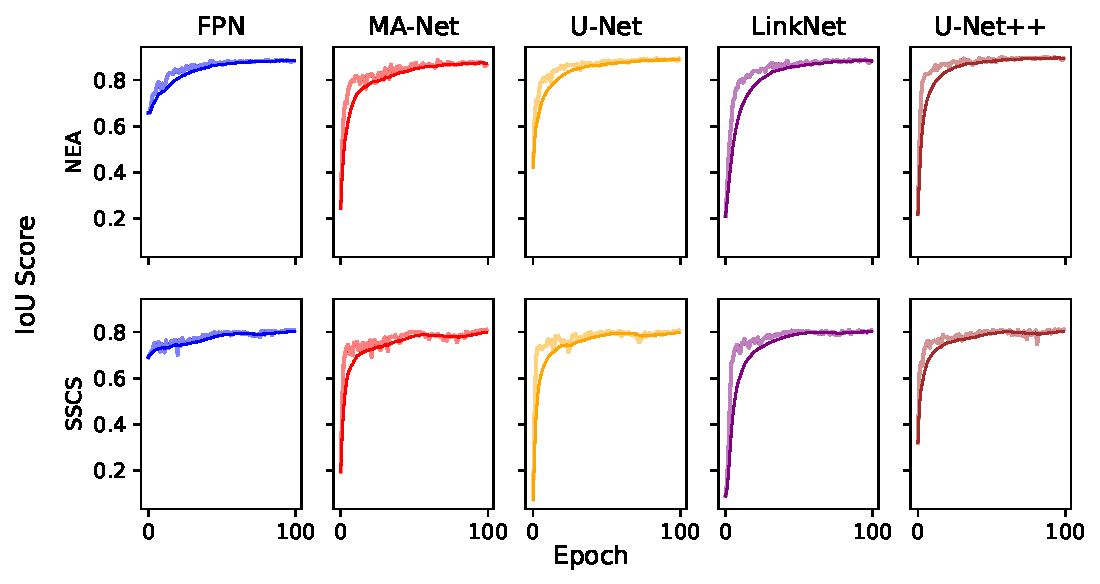
\includegraphics[width=0.9\textwidth]{figures/iou_training_progress.pdf}
    \caption{Validation IoU score on the first training stage}
    \label{fig:results:training:iou}
    \end{center}
\end{figure}

Afterward, we briefly describe the pruning
progress based on the validation \ac{iou} of
each combination of model, pruning algorithm
and sparsity. We choose several representative
figure to be shown in this figure, while 
the rest are accessible in the Github repository.
Figure~\ref{fig:results:pruning:iou} shows the validation
\ac{iou} obtained by the models throughout the pruning
stage and the fine-tuning stage. As previously described,
the fine-tuning starts after 50 epochs of pruning. 
Similar to Figure~\ref{fig:results:training:iou},
Figure~\ref{fig:results:pruning:iou} also shows
the actual and the exponential moving average values.

\begin{figure}[!ht]
    \centering
      \begin{subfigure}[t]{.29\textwidth}
        \centering
        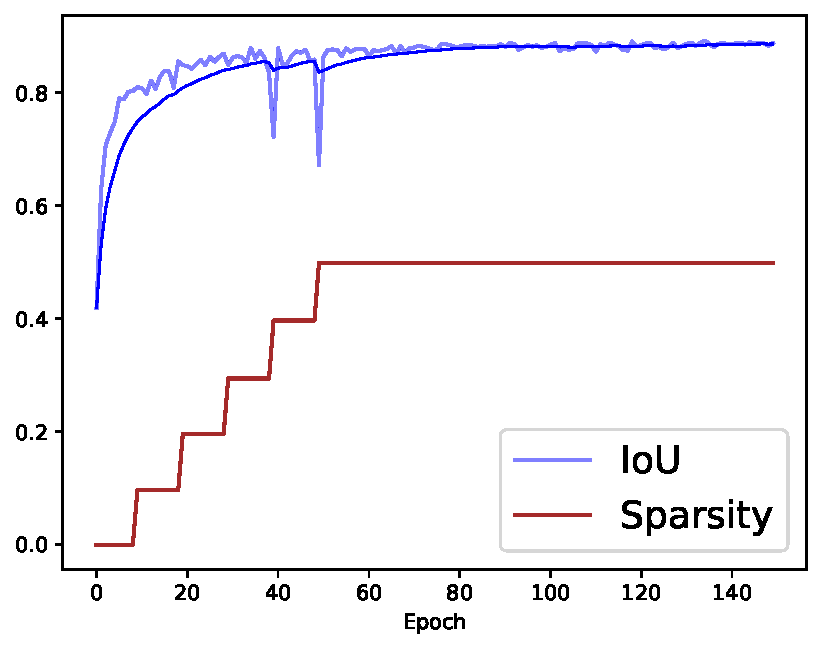
\includegraphics[width=.95\linewidth]{figures/pruning/unet_linear_0.5_NEAtraining_progress.pdf}
        \caption{U-Net, \ac{lp}, and $\zeta_f=0.5$ for \ac{nea} dataset}
        \label{fig:results:pruning:iou:unet-lp-0.5-nea}
      \end{subfigure}
      \hfill
      \begin{subfigure}[t]{.29\textwidth}
        \centering
        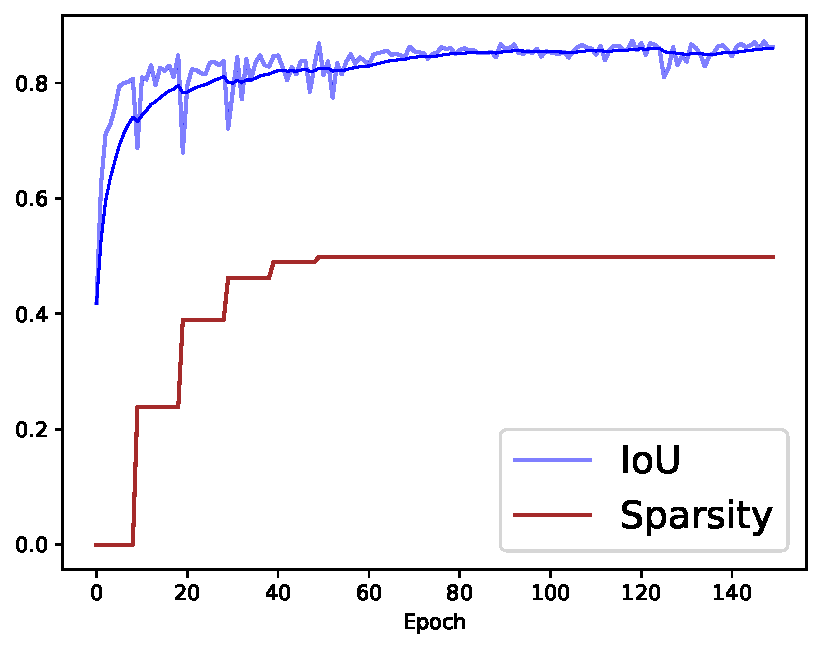
\includegraphics[width=.95\linewidth]{figures/pruning/unet_agp_0.5_NEAtraining_progress.pdf}
        \caption{U-Net, \ac{agp}, and $\zeta_f=0.5$ for \ac{nea} dataset}
        \label{fig:results:pruning:iou:unet-agp-0.5-nea}
      \end{subfigure}
      \hfill
      \begin{subfigure}[t]{.29\textwidth} 
        \centering
        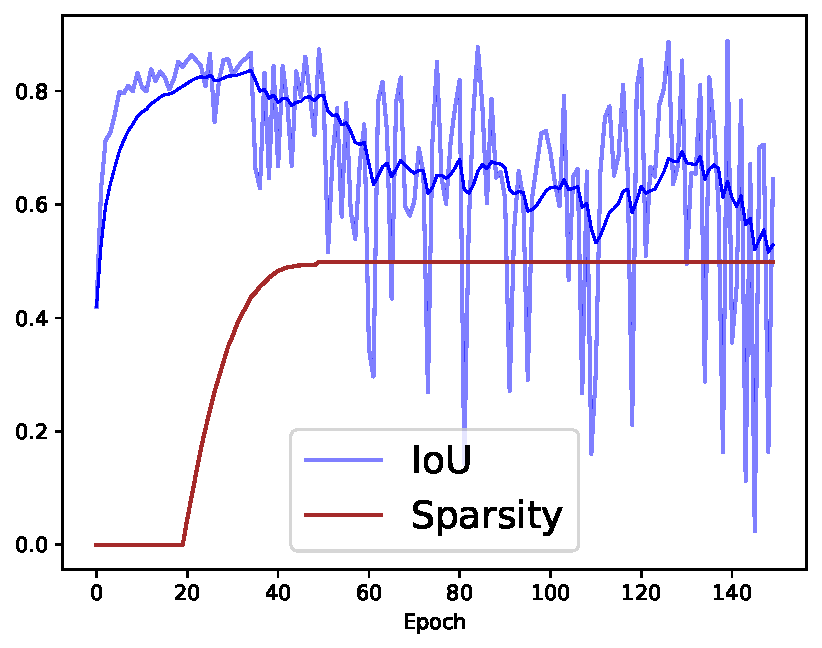
\includegraphics[width=.95\linewidth]{figures/pruning/unet_movement_0.5_NEAtraining_progress.pdf}
        \caption{U-Net, \ac{mp}, and $\zeta_f=0.5$ for \ac{nea} dataset}
        \label{fig:results:pruning:iou:unet-mp-0.5-nea}
      \end{subfigure}
      \vskip\baselineskip
      \begin{subfigure}[t]{.29\textwidth}
        \centering
        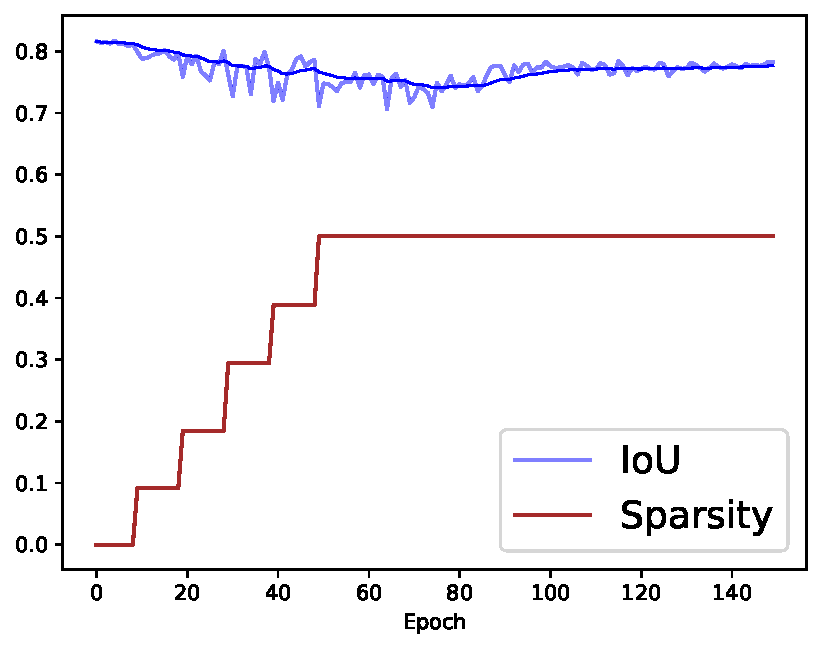
\includegraphics[width=.95\linewidth]{figures/pruning/fpn_linear_0.5_CCSCtraining_progress.pdf}
        \caption{\ac{fpn}, \ac{lp}, and $\zeta_f=0.5$ for \ac{sscs} dataset}
        \label{fig:results:pruning:iou:fpn-lp-0.5-sscs}
      \end{subfigure}
      \hfill
      \begin{subfigure}[t]{.29\textwidth}
        \centering
        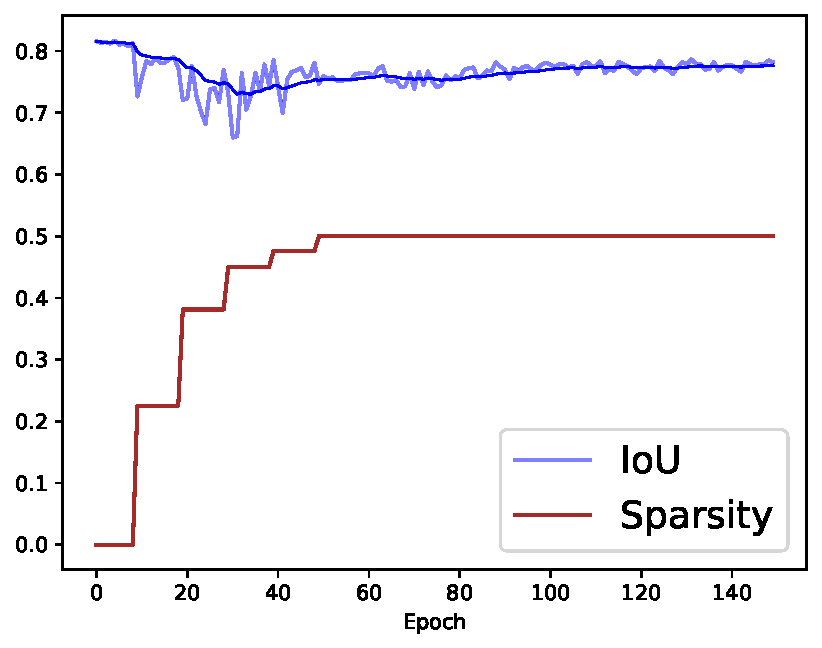
\includegraphics[width=.95\linewidth]{figures/pruning/fpn_agp_0.5_CCSCtraining_progress.pdf}
        \caption{\ac{fpn}, \ac{agp}, and $\zeta_f=0.5$ for \ac{sscs} dataset}
        \label{fig:results:pruning:iou:fpn-agp-0.5-sscs}
      \end{subfigure}
      \hfill
      \begin{subfigure}[t]{.29\textwidth}
        \centering
        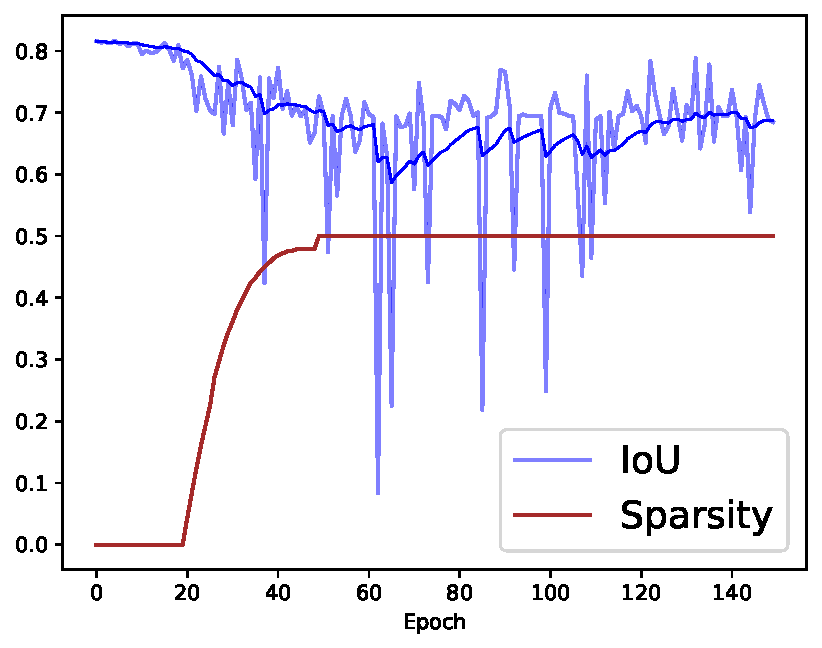
\includegraphics[width=.95\linewidth]{figures/pruning/fpn_movement_0.5_CCSCtraining_progress.pdf}
        \caption{\ac{fpn}, \ac{mp}, and $\zeta_f=0.5$ for \ac{sscs} dataset}
        \label{fig:results:pruning:iou:fpn-mp-0.5-sscs}
      \end{subfigure}
      \caption{The validation IoU in the pruning and fine-tuning stages}
      \label{fig:results:pruning:iou}
\end{figure}

Firstly, we can see that for \ac{lp} and \ac{agp},
the volatility in validation \ac{iou} is muchh less
compared to that of \ac{mp} in both models and datasets.
For \ac{lp} and \ac{agp}, there is a 
notable reduction in validation \ac{iou}
every $\Delta t$ or when the sparsity increases.
However, for $\zeta_f$, the validation \ac{iou}
can be retained and even improved after the fine-tuning phase.
On the other hand, we can notice very high volatility
in validation \ac{iou} when \ac{mp} is employed.
In addition, these great changes in validation \ac{iou}
not only occured in the pruning phase, but even more
in the fine-tuning phase where the sparsity
of the model is retained. Therefore, we
can denote that based on the validation \ac{iou},
\ac{lp} and \ac{agp} are preferred because they can
better retain the models' performance 
after pruning and have a more stable learning process.

Finally, we will evaluate the performance of
each combination of model and pruner based on
the achieved \ac{iou} on the testing dataset
as shown in Figure~\ref{fig:results:test:nea}
and Figure~\ref{fig:results:test:sscs}. Several
noteworthy observations can be made on the
two figures. Firstly, for \ac{agp} and \ac{lp},
the achieved \ac{iou} decreases as $\zeta_f$
increases. We can also note that
\ac{fpn} and LinkNet best retain \ac{iou}
on $\zeta_f=0.9$ compared to the other models
on \ac{sscs} dataset with \ac{agp} and \ac{lp}.
Meanwhile, on \ac{nea}
dataset, U-Net and \ac{fpn} best retain \ac{iou}
on $\zeta_f=0.9$ with \ac{agp}, while LinkNet and
U-Net best retain \ac{iou} with \ac{lp}.


\begin{figure}[!ht]
    \centering
      \begin{subfigure}[t]{.292\textwidth}
        \centering
        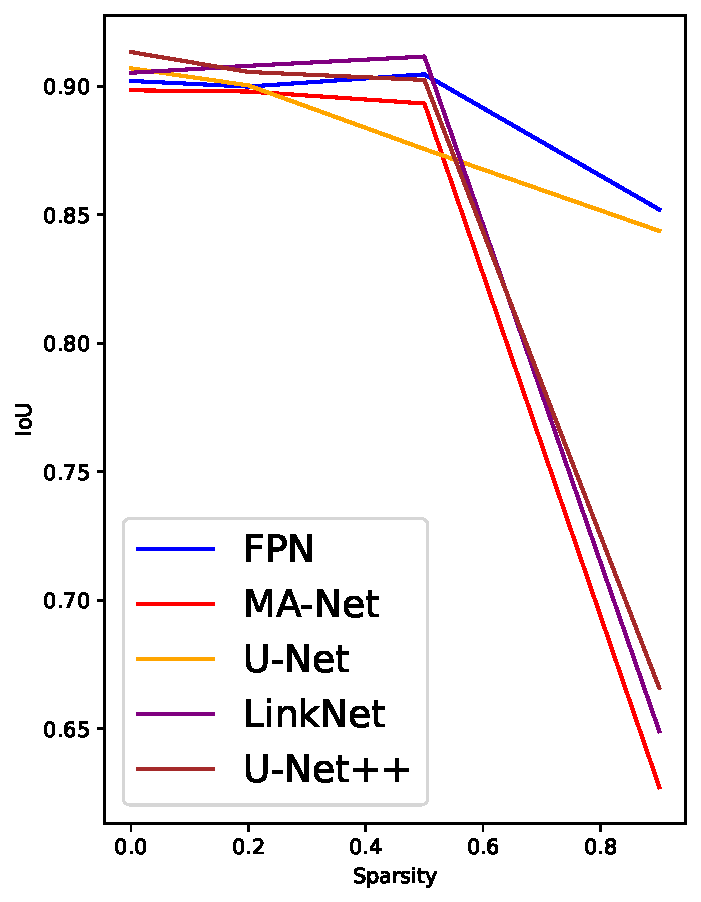
\includegraphics[width=.95\linewidth]{figures/test/pruning-testing-score_NEA_agp.pdf}
        \caption{\ac{agp}}
        \label{fig:results:test:nea:agp}
      \end{subfigure}
      \hfill
      \begin{subfigure}[t]{.28\textwidth}
        \centering
        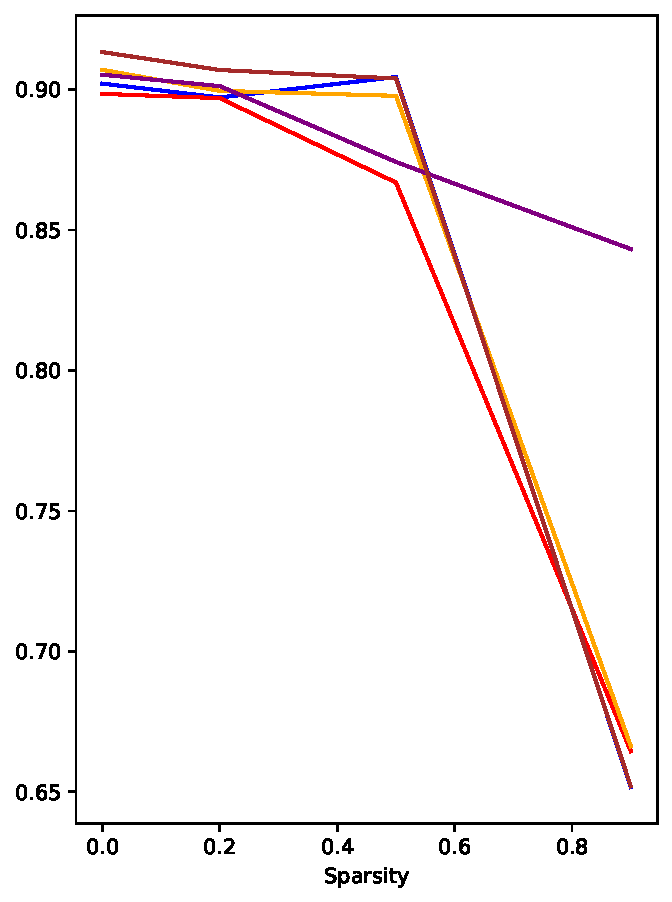
\includegraphics[width=.95\linewidth]{figures/test/pruning-testing-score_NEA_linear.pdf}
        \caption{\ac{lp}}
        \label{fig:results:test:nea:lp}
      \end{subfigure}
      \hfill
      \begin{subfigure}[t]{.276\textwidth} 
        \centering
        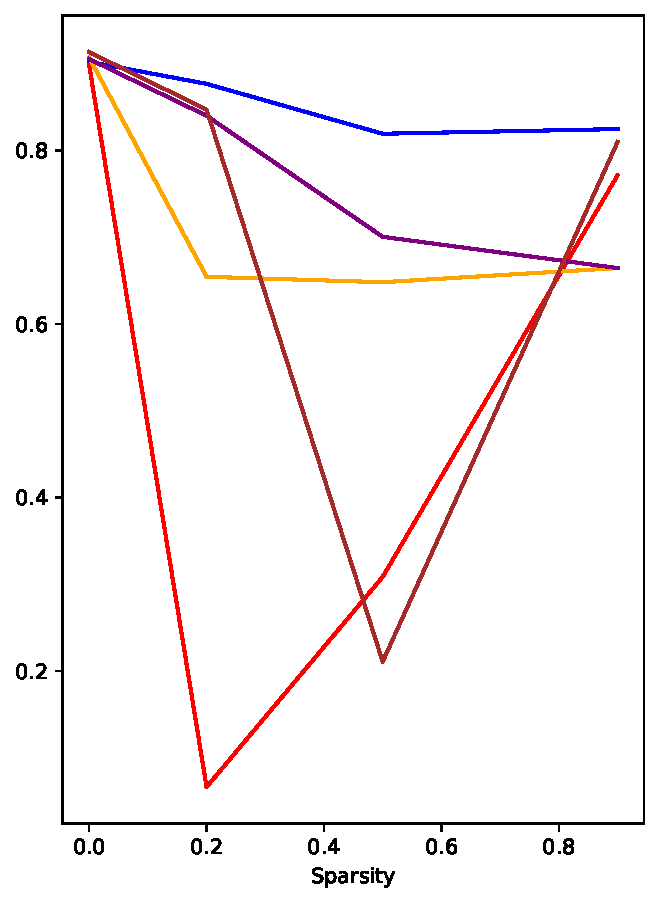
\includegraphics[width=.95\linewidth]{figures/test/pruning-testing-score_NEA_movement.pdf}
        \caption{\ac{mp}}
        \label{fig:results:test:nea:mp}
      \end{subfigure}
      \caption{The testing IoU for various pruning algorithms in increasing sparsity on NEA dataset}
      \label{fig:results:test:nea}
\end{figure}

\begin{figure}[!ht]
    \centering
      \begin{subfigure}[t]{.294\textwidth}
        \centering
        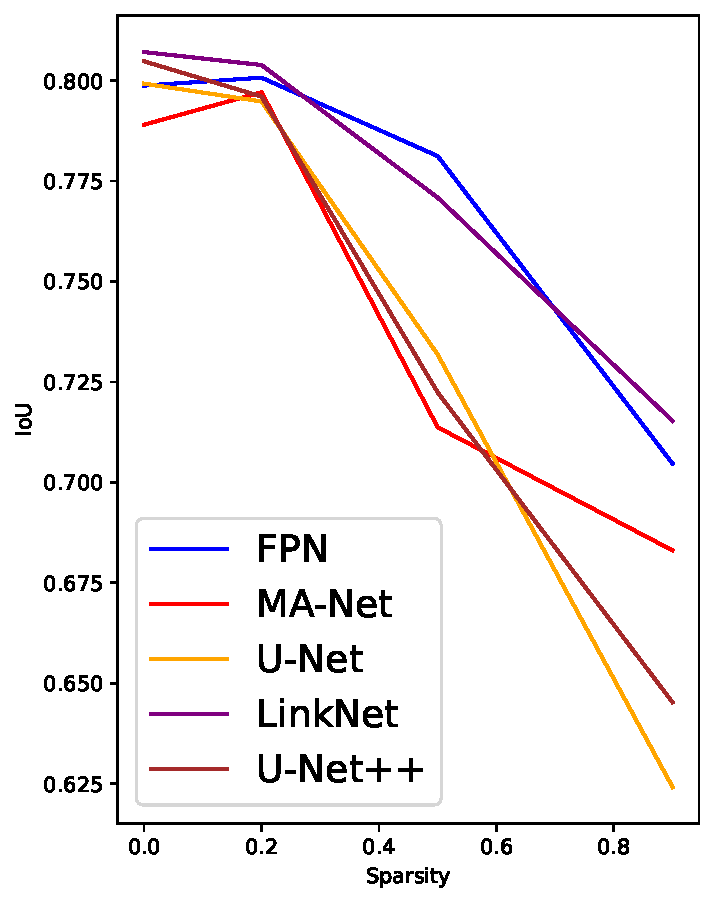
\includegraphics[width=.95\linewidth]{figures/test/pruning-testing-score_CCSC_agp.pdf}
        \caption{\ac{agp}}
        \label{fig:results:test:sscs:agp}
      \end{subfigure}
      \hfill
      \begin{subfigure}[t]{.284\textwidth}
        \centering
        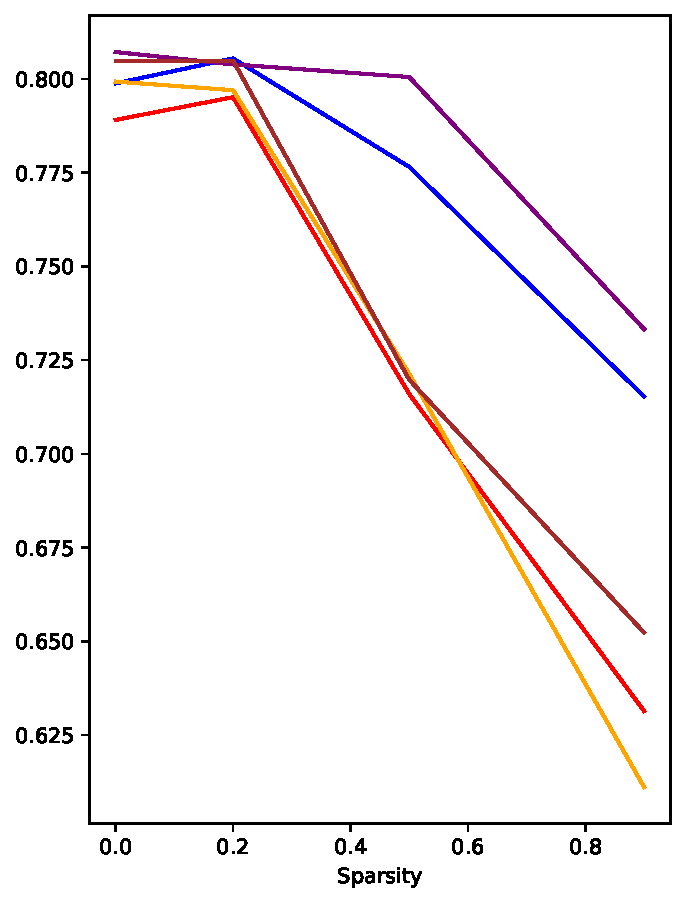
\includegraphics[width=.95\linewidth]{figures/test/pruning-testing-score_CCSC_linear.pdf}
        \caption{\ac{lp}}
        \label{fig:results:test:sscs:lp}
      \end{subfigure}
      \hfill
      \begin{subfigure}[t]{.274\textwidth} 
        \centering
        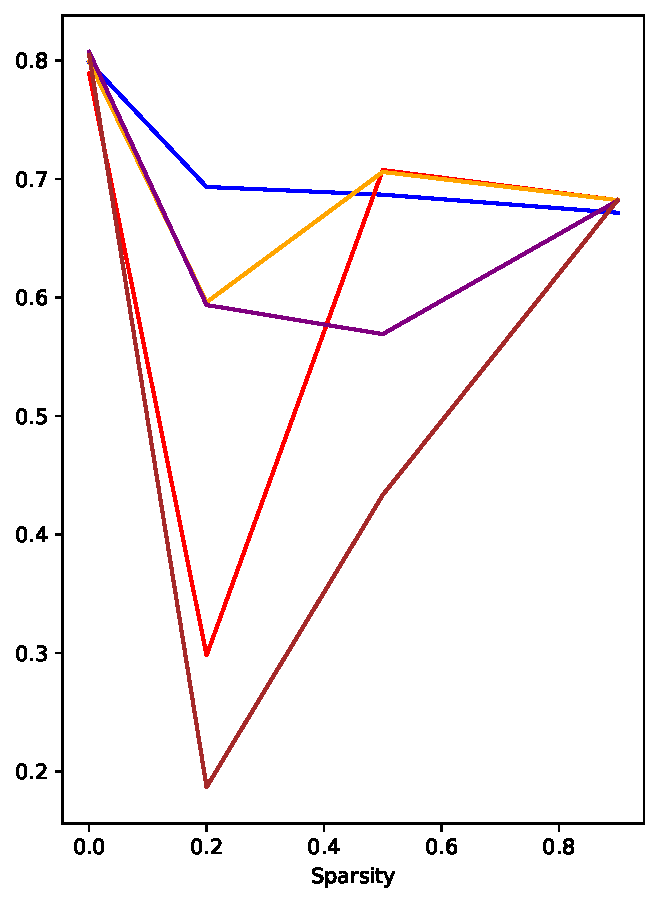
\includegraphics[width=.95\linewidth]{figures/test/pruning-testing-score_CCSC_movement.pdf}
        \caption{\ac{mp}}
        \label{fig:results:test:sscs:mp}
      \end{subfigure}
      \caption{The testing IoU for various pruning algorithms in increasing sparsity on SSCS dataset}
      \label{fig:results:test:sscs}
\end{figure}

Interestingly, it can be observed on both \ac{nea}
and \ac{sscs} datasets, \ac{mp} retains
better \ac{iou} with all models on $\zeta_f=0.9$
compared to \ac{agp} and \ac{lp}.
However, contrary to \ac{agp} and \ac{lp},
the \ac{iou} achieved by the models pruned by \ac{mp}
is the lowest on $\zeta_f=0.2$. 
Therefore, a further experimental study
needs to be conducted to determine the cause
of extremely low achieved \ac{iou} for \ac{mp}
on $\zeta_f=0.2$. This experimental study
can include hyperparamater tuning for the pruning phase
and fine-tuning phase, and a more granular
choice of $\zeta_f$. We leave these additional experimental
evaluations for our future study.

Lastly, we will show representative examples
of the predicted labels generated by the pruned
models. Other visualizations are provided in the GitHub repository.
Figure~\ref{fig:results:pruning:visualization:nea} 
shows the labels generated by \ac{fpn} 
with varying sparsity with the three pruning methods. 
The displayed figures
can represent the difference in testing \ac{iou}
previously described. As can be observed, 
using \ac{agp} or \ac{lp},
the generated label mask up to $\zeta_f=0.5$ is
still very similar compared to the initial label mask,
which is resembled by the testing \ac{iou}
that is retained up to $\zeta_f=0.5$. 
On the other hand, the model pruned with \ac{mp}
with $\zeta_f=0.5$ generates significantly different
label mask, where some poor labels are missing and
some severe areas are misclassified as poor areas.
For models pruned up to $\zeta_f=0.9$, where 
the testing \ac{iou} deteriorates significantly, 
we can observed that all models can only classify
the pixels into only one class. \ac{agp} and \ac{mp}
classified all corroded areas into severe areas,
while \ac{lp} classified all into poor areas. Most
corroded areas are severe areas, therefore 
the models pruned by \ac{agp} and \ac{mp}
have more pixels correctly labeled, compared to the model
pruned by \ac{lp}. This explains 
why \ac{lp} has the worst testing \ac{iou} on
$\zeta_f=0.9$ compared to \ac{agp} and \ac{mp}.

\begin{figure}[!ht]
    \centering
      \begin{subfigure}[t]{.4\textwidth}
        \centering
        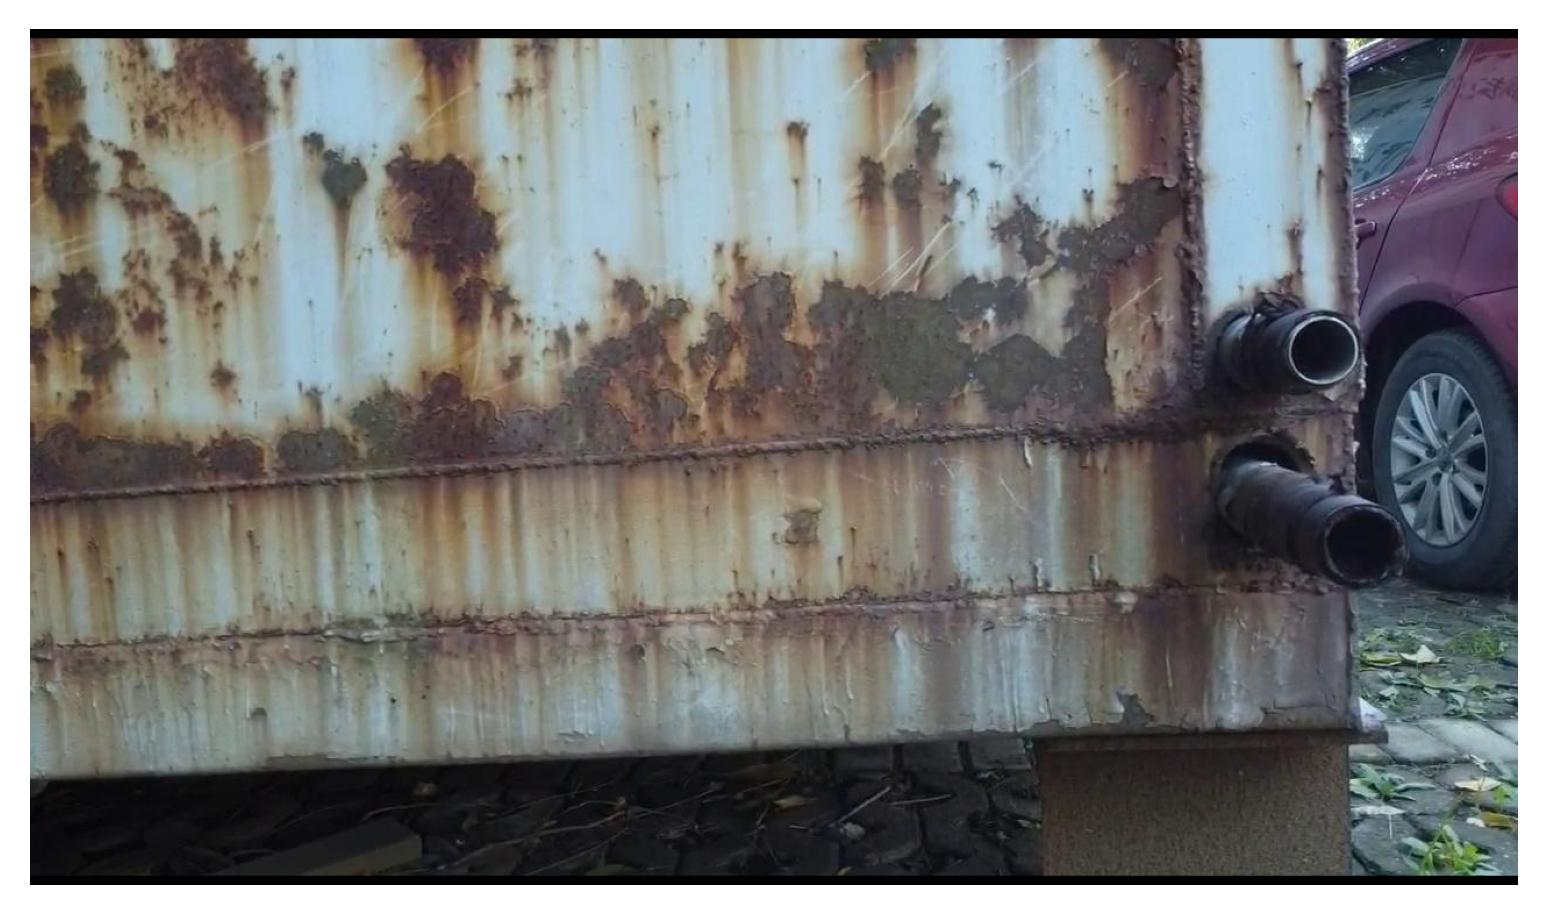
\includegraphics[width=.95\linewidth]{figures/pruning-results/NEA/11.jpg}
        \caption{Example image}
        \label{fig:results:pruning:visualization:nea-fpn-x}
      \end{subfigure}
    %   \hfill
      \begin{subfigure}[t]{.4\textwidth}
        \centering
        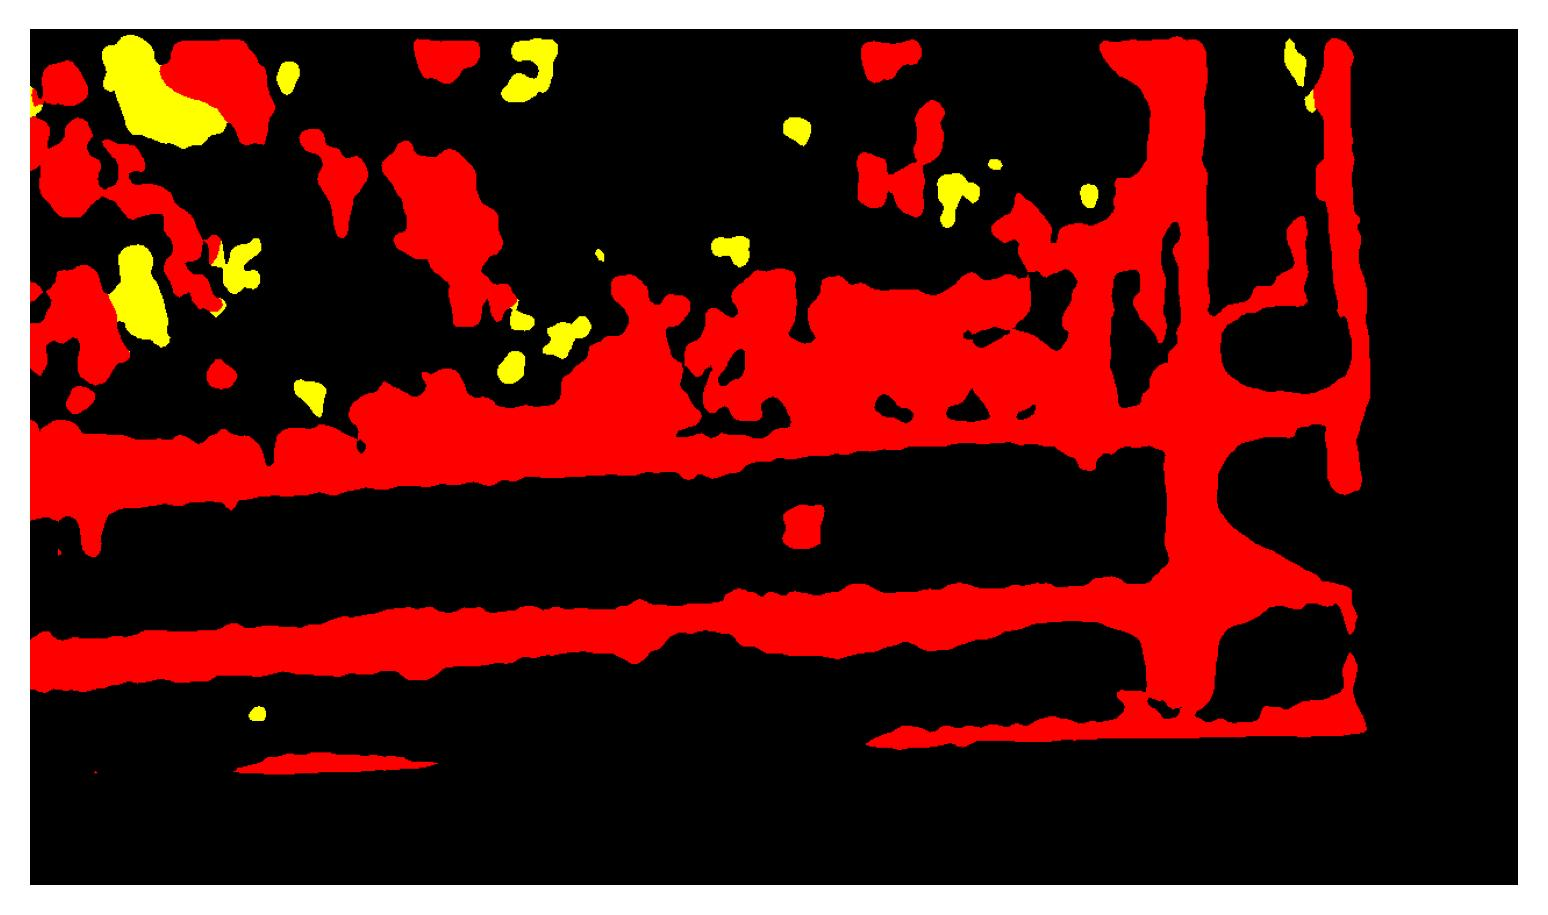
\includegraphics[width=.95\linewidth]{figures/pruning-results/fpn_NEA_agp/10/mask_0.jpg}
        \caption{Label mask generated by \ac{fpn}}
        \label{fig:results:pruning:visualization:nea-fpn}
      \end{subfigure}
      \vskip\baselineskip
      \begin{subfigure}[t]{.29\textwidth} 
        \centering
        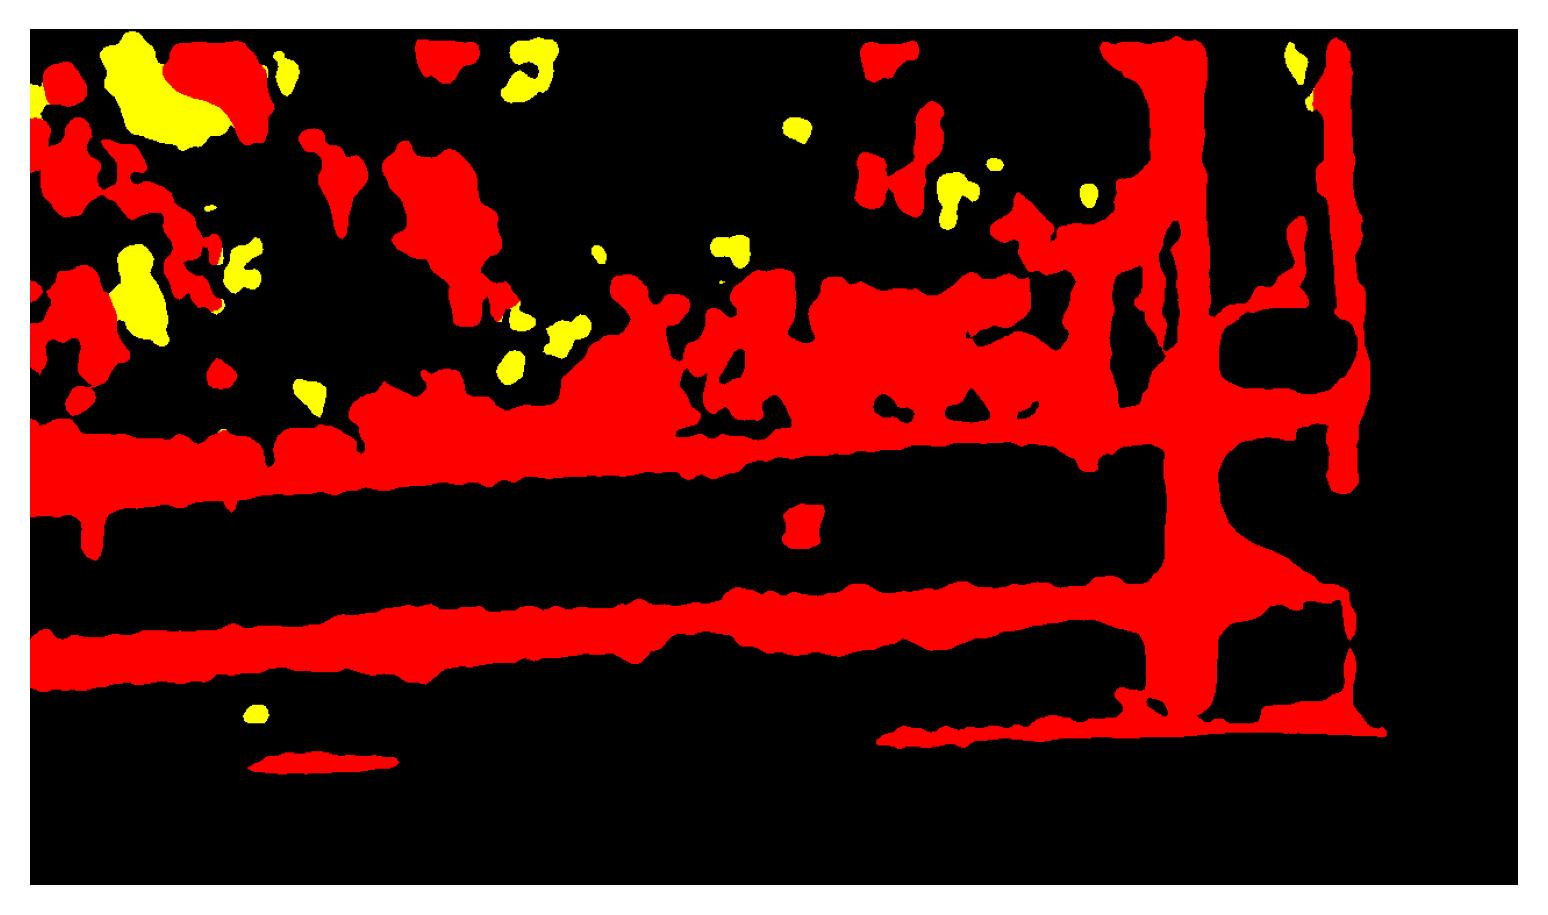
\includegraphics[width=.95\linewidth]{figures/pruning-results/fpn_NEA_agp/10/mask_0.2.jpg}
        \caption{\ac{agp}, $\zeta_f=0.2$}
        \label{fig:results:pruning:visualization:nea-fpn-agp-0.2}
      \end{subfigure} 
      \begin{subfigure}[t]{.29\textwidth} 
        \centering
        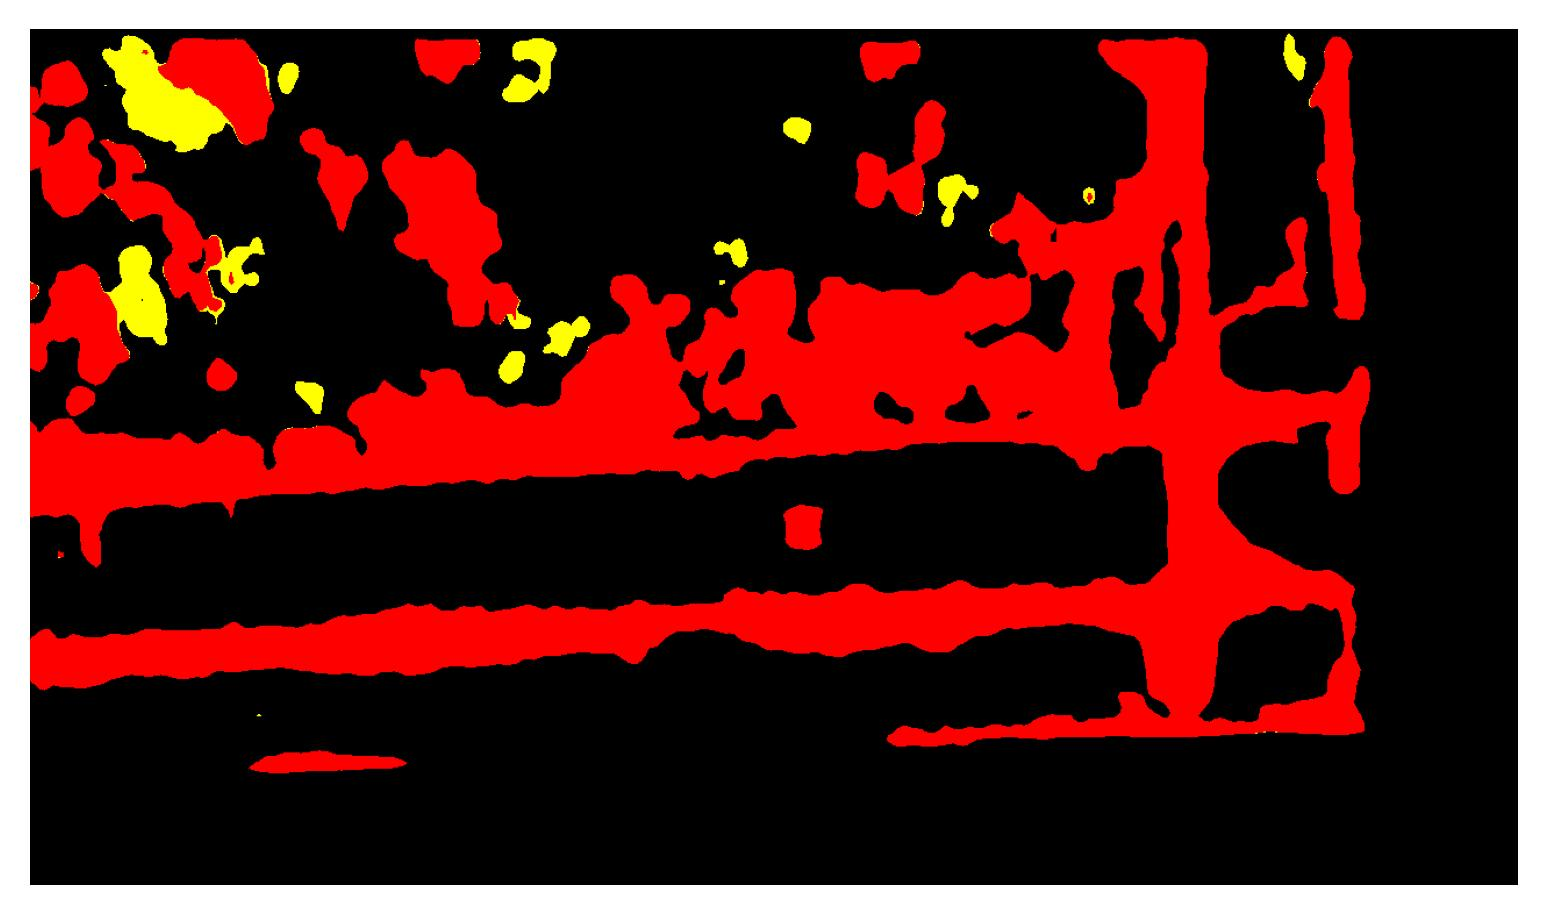
\includegraphics[width=.95\linewidth]{figures/pruning-results/fpn_NEA_agp/10/mask_0.5.jpg}
        \caption{\ac{agp}, $\zeta_f=0.5$}
        \label{fig:results:pruning:visualization:nea-fpn-agp-0.5}
      \end{subfigure}
      \begin{subfigure}[t]{.29\textwidth} 
        \centering
        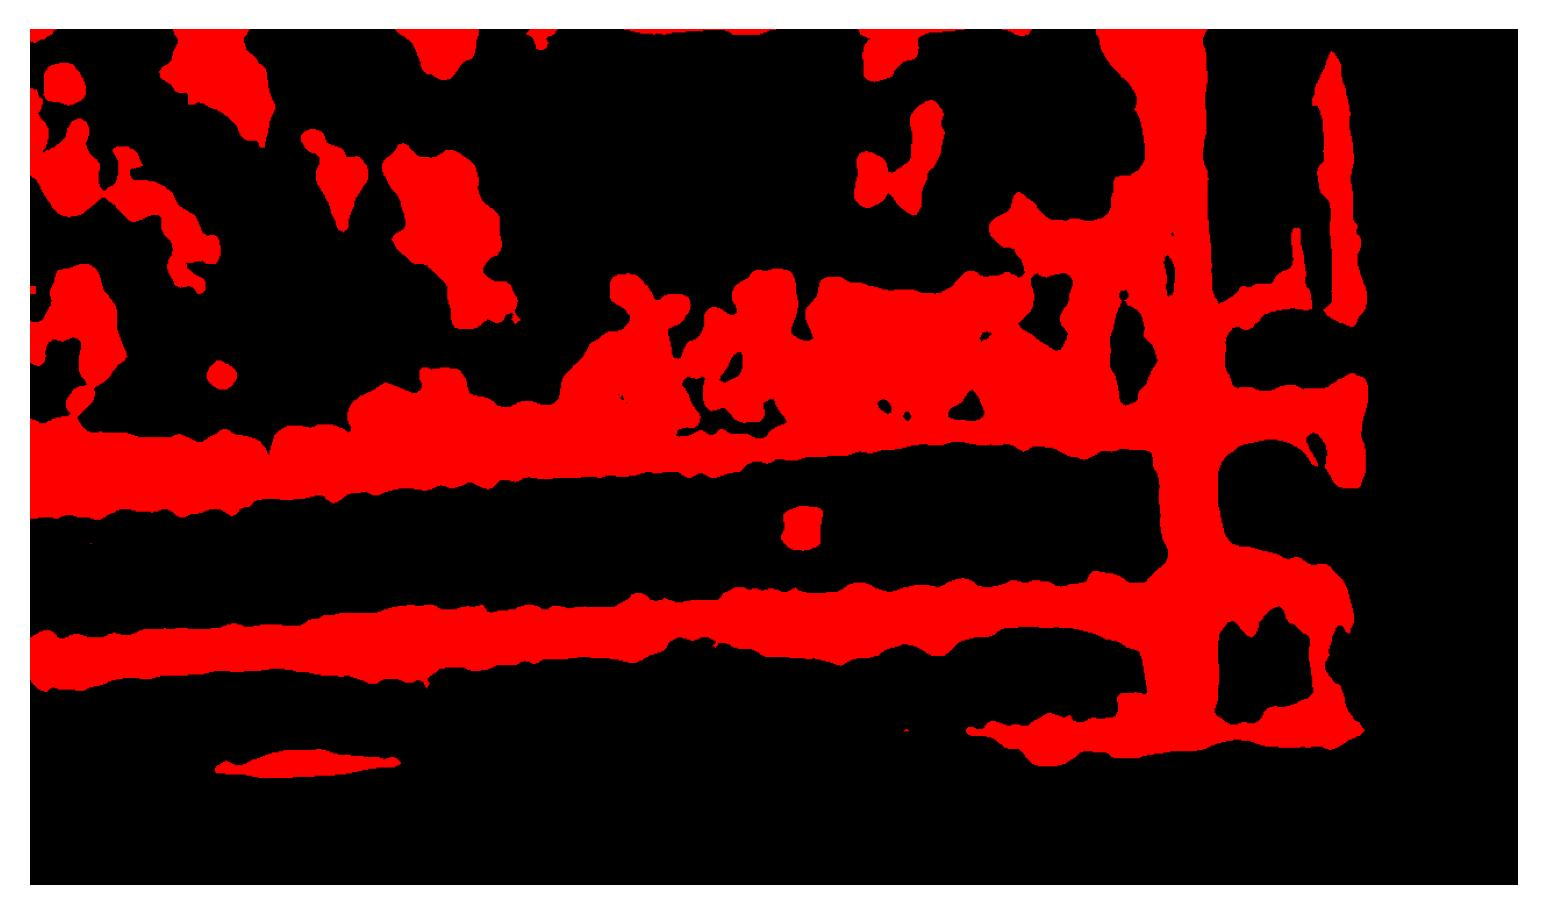
\includegraphics[width=.95\linewidth]{figures/pruning-results/fpn_NEA_agp/10/mask_0.9.jpg}
        \caption{\ac{agp}, $\zeta_f=0.9$}
        \label{fig:results:pruning:visualization:nea-fpn-agp-0.9}
      \end{subfigure}
      \vskip\baselineskip
      \begin{subfigure}[t]{.29\textwidth} 
        \centering
        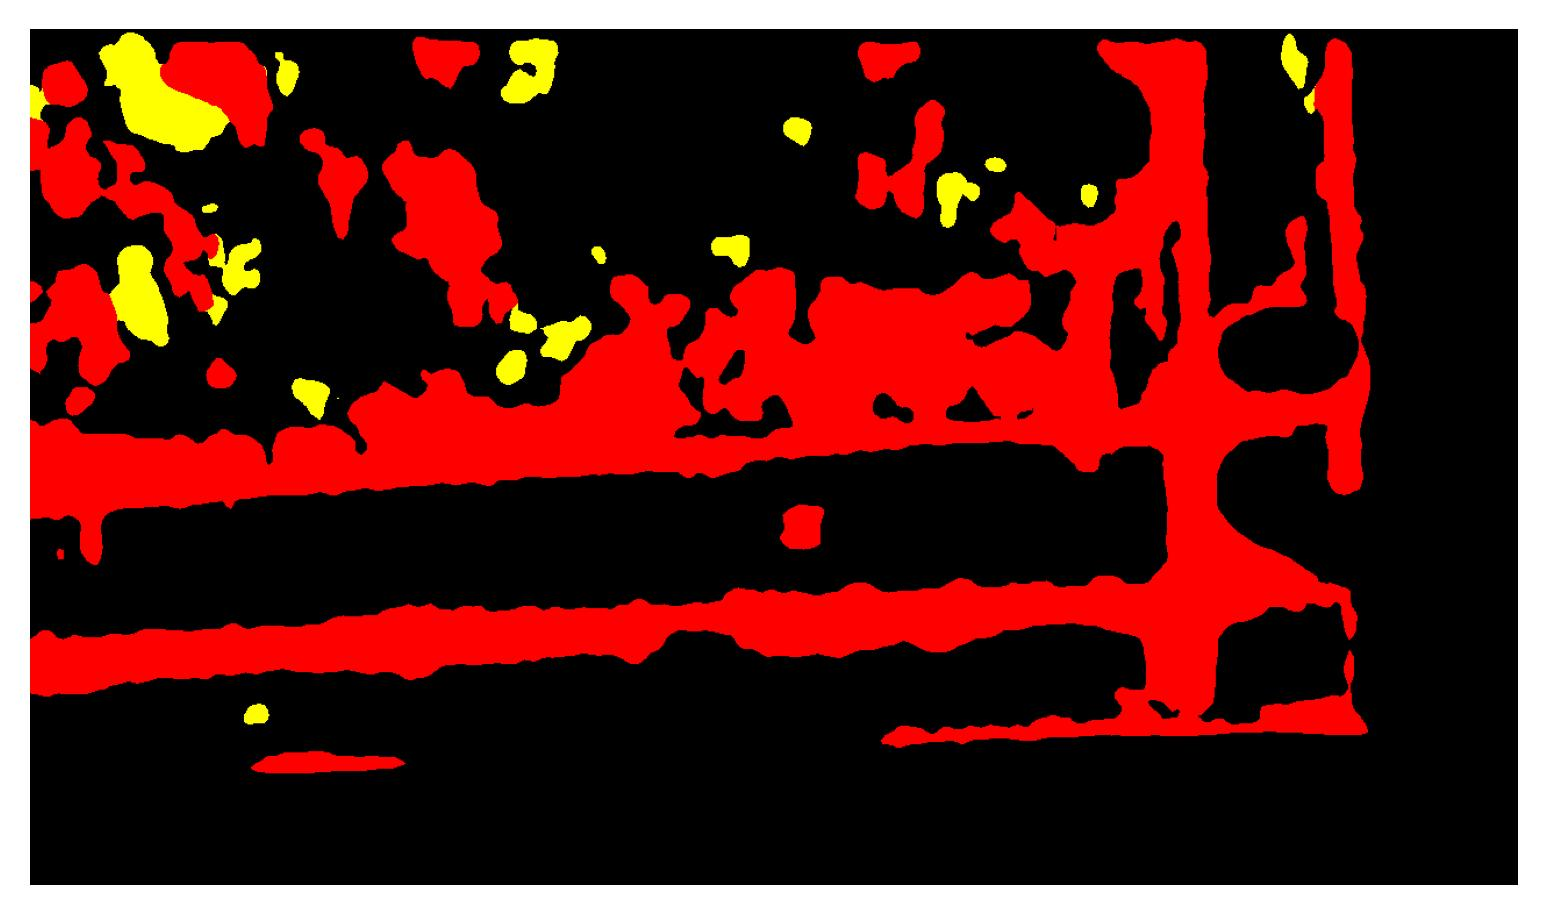
\includegraphics[width=.95\linewidth]{figures/pruning-results/fpn_NEA_linear/10/mask_0.2.jpg}
        \caption{\ac{lp}, $\zeta_f=0.2$}
        \label{fig:results:pruning:visualization:nea-fpn-lp-0.2}
      \end{subfigure}
      \begin{subfigure}[t]{.29\textwidth} 
        \centering
        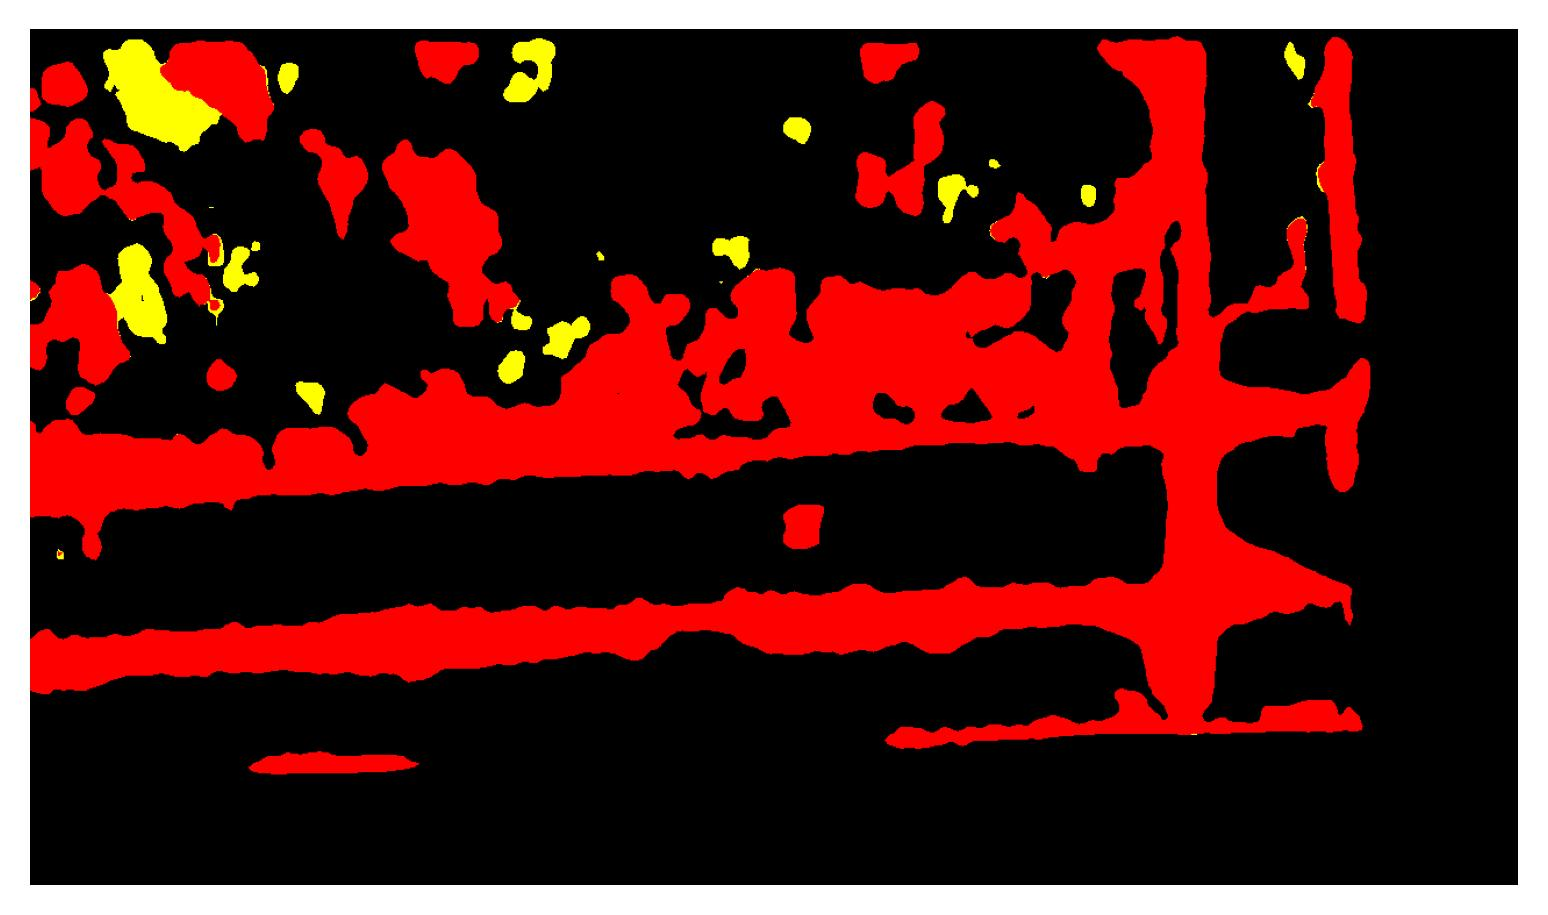
\includegraphics[width=.95\linewidth]{figures/pruning-results/fpn_NEA_linear/10/mask_0.5.jpg}
        \caption{\ac{lp}, $\zeta_f=0.5$}
        \label{fig:results:pruning:visualization:nea-fpn-lp-0.5}
      \end{subfigure}
      \begin{subfigure}[t]{.29\textwidth} 
        \centering
        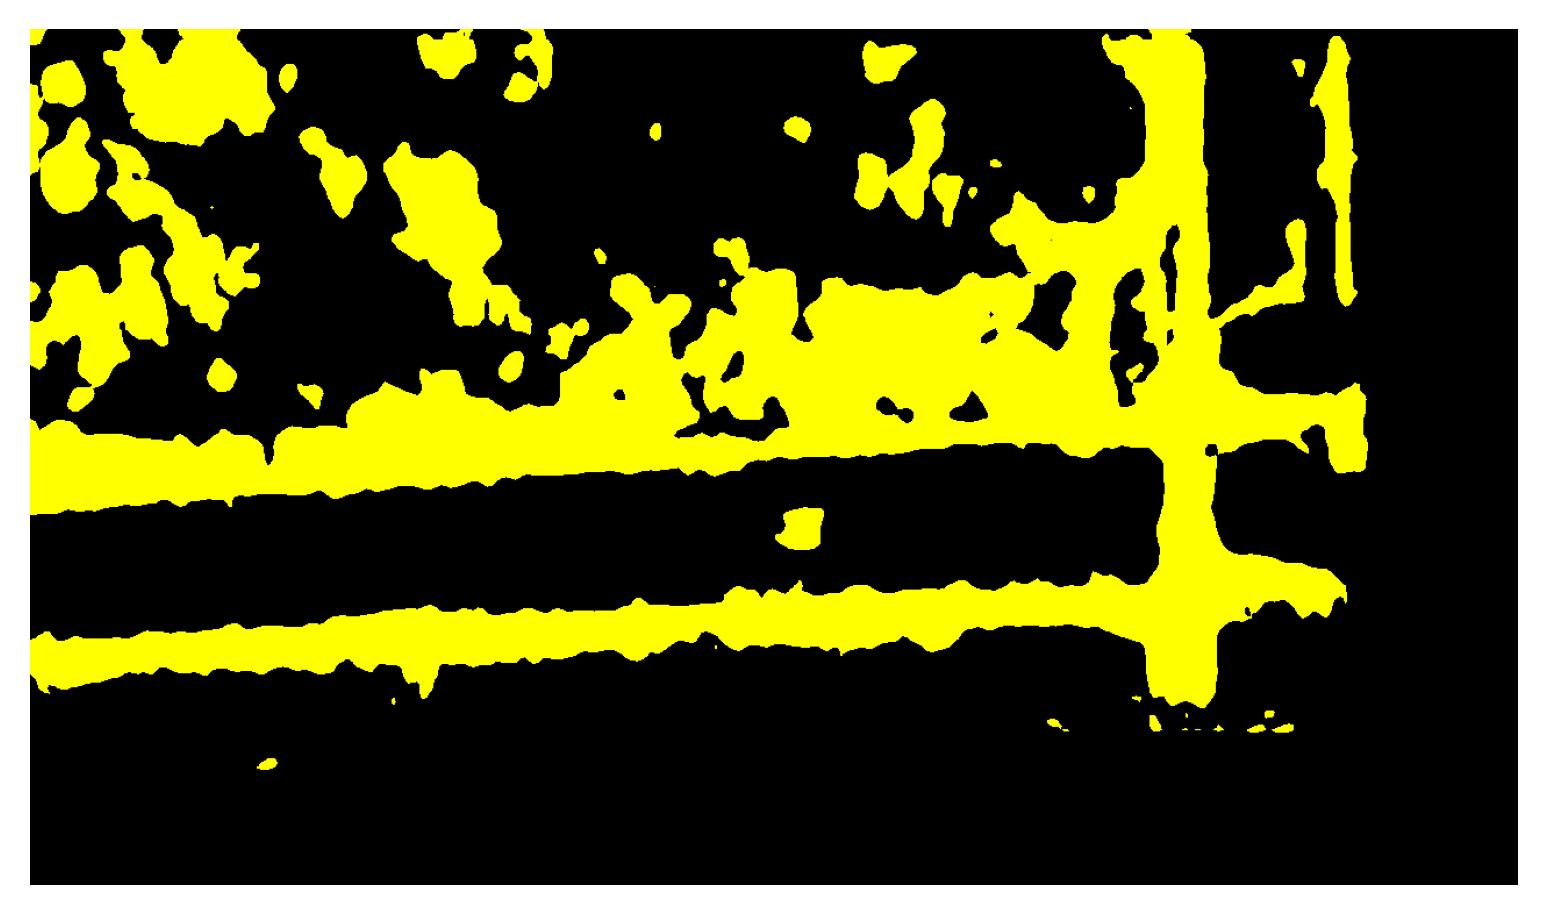
\includegraphics[width=.95\linewidth]{figures/pruning-results/fpn_NEA_linear/10/mask_0.9.jpg}
        \caption{\ac{lp}, $\zeta_f=0.9$}
        \label{fig:results:pruning:visualization:nea-fpn-lp-0.9}
      \end{subfigure}
      \vskip\baselineskip
      \begin{subfigure}[t]{.29\textwidth} 
        \centering
        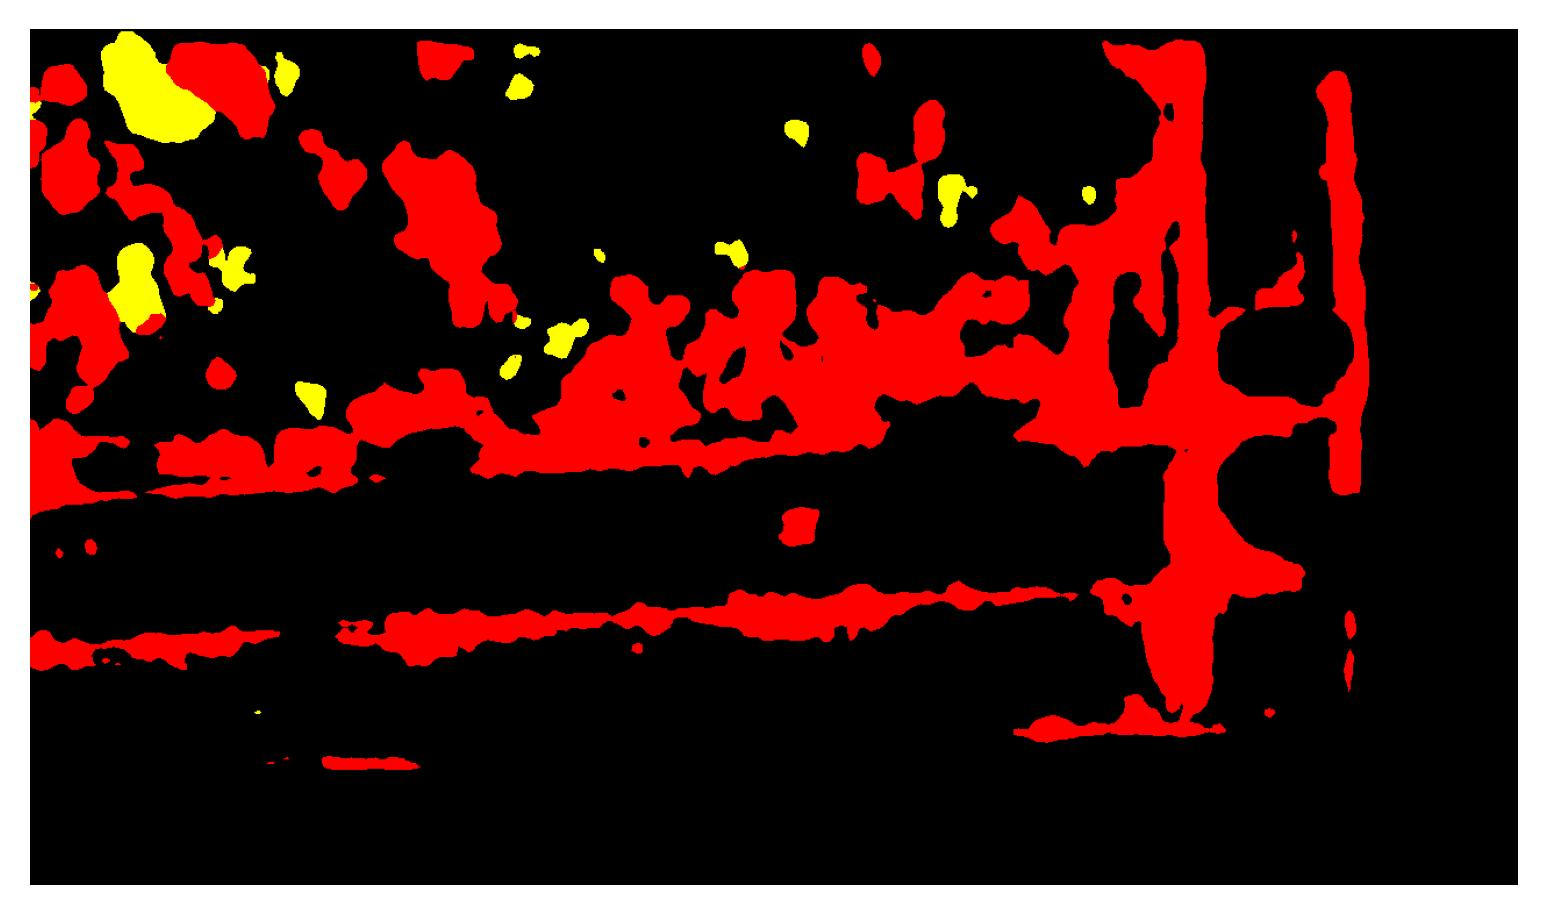
\includegraphics[width=.95\linewidth]{figures/pruning-results/fpn_NEA_movement/10/mask_0.2.jpg}
        \caption{\ac{mp}, $\zeta_f=0.2$}
        \label{fig:results:pruning:visualization:nea-fpn-mp-0.2}
      \end{subfigure}
      \begin{subfigure}[t]{.29\textwidth} 
        \centering
        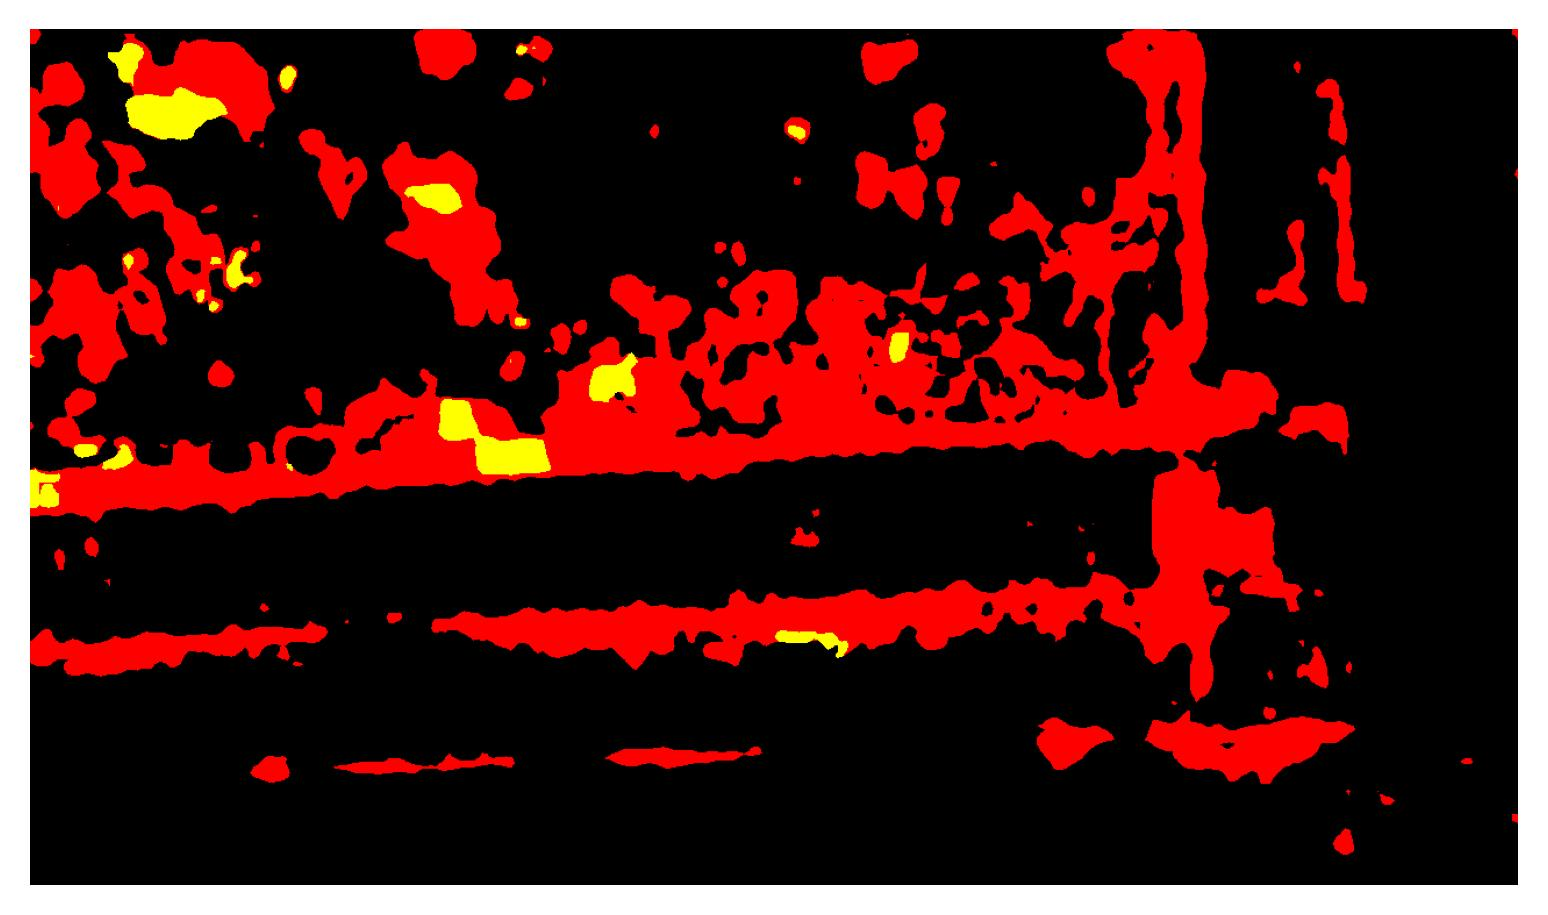
\includegraphics[width=.95\linewidth]{figures/pruning-results/fpn_NEA_movement/10/mask_0.5.jpg}
        \caption{\ac{mp}, $\zeta_f=0.5$}
        \label{fig:results:pruning:visualization:nea-fpn-mp-0.5}
      \end{subfigure}
      \begin{subfigure}[t]{.29\textwidth} 
        \centering
        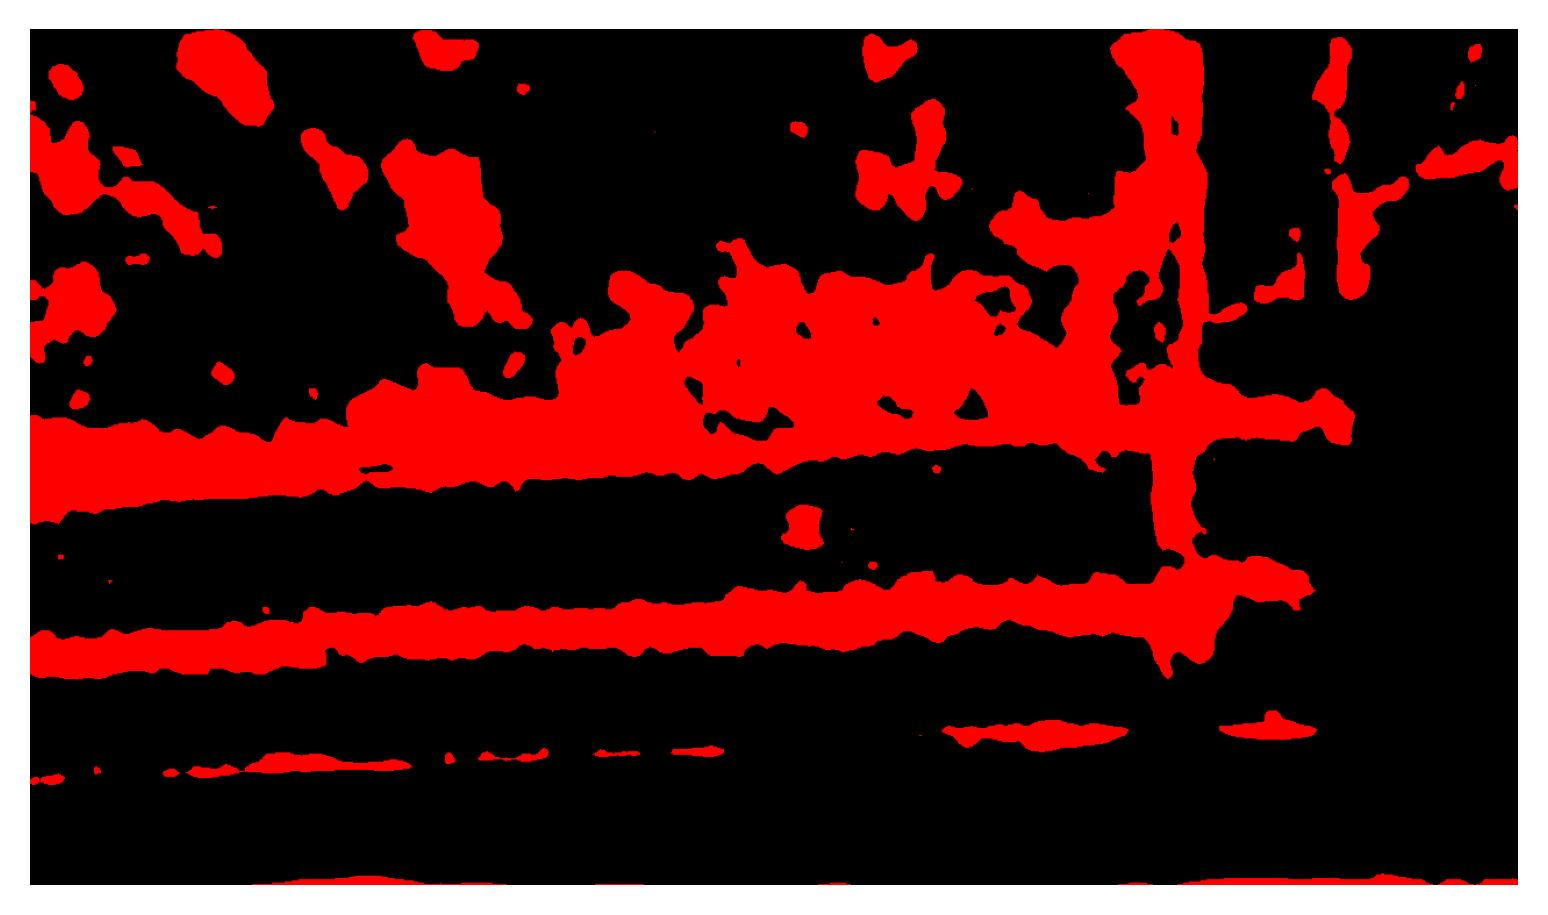
\includegraphics[width=.95\linewidth]{figures/pruning-results/fpn_NEA_movement/10/mask_0.9.jpg}
        \caption{\ac{mp}, $\zeta_f=0.9$}
        \label{fig:results:pruning:visualization:nea-fpn-mp-0.9}
      \end{subfigure}
      \caption{Example of image and the label mask generated by FPN on NEA dataset}
      \label{fig:results:pruning:visualization:nea}
  \end{figure}

% \begin{figure}[htbp]
%     \begin{center}
%     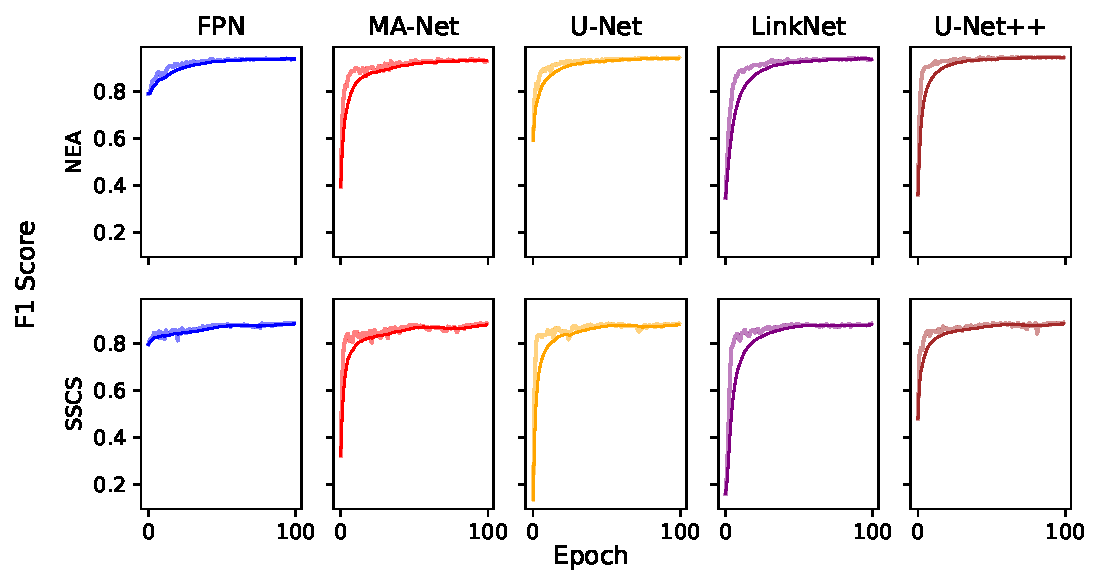
\includegraphics[width=0.9\textwidth]{figures/f1_training_progress.pdf}
%     \caption{Validation F1 score on the first training stage}
%     \label{fig:results:training:f1}
%     \end{center}
% \end{figure}
These results indicate that we can produce lightweight
metal corrosion segmentation models by the training, 
pruning and fine-tuning framework as is done in this study.
We have shown that the models, especially \ac{fpn},
and LinkNet, can be pruned with \ac{agp}
and \ac{lp} up to $\zeta_f=0.5$ without
significant reduction in performance. Further study
is needed to improve the performance of the models
if we aim to prune the models up to $\zeta_f=0.9$. 

In addition to a more comprehensive experimental study,
the model performance, as well as the quality of future
studies, can be greatly improved by expanding and improving
the quality of the metal corrosion image dataset.
Despite the importance of metal corrosion image dataset


\section{Conclusions}
In this study, we have trained and evaluated five 
segmentation models, i.e., \ac{fpn}, U-Net, U-Net++, 
LinkNet and \ac{manet}. The results indicate that for 
these two datasets, \ac{fpn} and LinkNet perform better compared to 
the other three trained models.
The models can be pruned, especially with \ac{lp}
and \ac{agp}, up to $\zeta_f=0.5$ or 50\% of 
the parameters are removed with
little reduction in performance compared to
the original trained model. However,
the performance of the model deteriorates significantly
when pruned up to $\zeta_f=0.9$ with all three pruning
algorithms. This suggests that further analysis
and study are needed to improve the performance
of the models if we aim to prune the model up to $\zeta_f=0.9$.
This future study can include hyperparamater tuning
for the fine-tuning stage, more granular choice
of $\zeta_f$ to fine the sweet spot of sparsity
and performance, and evaluating other pruning algorithms.
In addition, further study can also aim to expand
the very limited dataset on 
metal corrosion image segmentation.

\reftitle{References}

% Please provide either the correct journal abbreviation (e.g. according to the “List of Title Word Abbreviations” http://www.issn.org/services/online-services/access-to-the-ltwa/) or the full name of the journal.
% Citations and References in Supplementary files are permitted provided that they also appear in the reference list here. 

%=====================================
% References, variant A: external bibliography
%=====================================
\bibliography{references}

%=====================================
% References, variant B: internal bibliography
%=====================================


% If authors have biography, please use the format below
%\section*{Short Biography of Authors}
%\bio
%{\raisebox{-0.35cm}{\includegraphics[width=3.5cm,height=5.3cm,clip,keepaspectratio]{Definitions/author1.pdf}}}
%{\textbf{Firstname Lastname} Biography of first author}
%
%\bio
%{\raisebox{-0.35cm}{\includegraphics[width=3.5cm,height=5.3cm,clip,keepaspectratio]{Definitions/author2.jpg}}}
%{\textbf{Firstname Lastname} Biography of second author}

% For the MDPI journals use author-date citation, please follow the formatting guidelines on http://www.mdpi.com/authors/references
% To cite two works by the same author: \citeauthor{ref-journal-1a} (\citeyear{ref-journal-1a}, \citeyear{ref-journal-1b}). This produces: Whittaker (1967, 1975)
% To cite two works by the same author with specific pages: \citeauthor{ref-journal-3a} (\citeyear{ref-journal-3a}, p. 328; \citeyear{ref-journal-3b}, p.475). This produces: Wong (1999, p. 328; 2000, p. 475)

%%%%%%%%%%%%%%%%%%%%%%%%%%%%%%%%%%%%%%%%%%
%% for journal Sci
%\reviewreports{\\
%Reviewer 1 comments and authors’ response\\
%Reviewer 2 comments and authors’ response\\
%Reviewer 3 comments and authors’ response
%}
%%%%%%%%%%%%%%%%%%%%%%%%%%%%%%%%%%%%%%%%%%
% \PublishersNote{}
\end{document}

